\documentclass[oneside,12pt]{Classes/VTU}
\title{Prediction of heart disease and diabetes using machine learning}
\author{by \\ \vspace{1mm}
\begin{tabular}{ccc}
\textbf{Akshat Agarwal }&  & \textbf{1SI16CS010}\\
\textbf{Akarsh Singh }&  & \textbf{1SI16CS007}\\
\textbf{Ayush Bhargava }&  & \textbf{1SI16CS131}\\
\textbf{Srijan Yadav }&  & \textbf{1SI16CS109}\\
\end{tabular}
\vspace{7mm} \\under the guidance of\\\textbf{H.K Vedamurthy}
\\Assistant Professor \vspace{0.5cm}}
%for Associate Professor - Associate Professor
%for Professor - Professor

\collegeordept{Department of Computer Science and Engineering}
\university{Siddaganga Institute of Technology, Tumakuru}

\renewcommand{\submittedtext}{A project report submitted to \\Visvesvaraya Technological University. Belgaum, Karnataka \\\textit{in the partial fulfillment of the requirements for the award of degree of} }
\degree{\textbf{\textit{Bachelor of Engineering}} \\ in \\ \textbf{\textit{Computer Science and Engineering}}}
\degreedate{\textbf{May, 2020}}

\hbadness=10000
\hfuzz=50pt

\usepackage[inner=1.2in, outer=1in, top=1.2in, bottom=1.2in]{geometry}

\date{2020}

%\setcounter{tocdepth}{3}
%\setcounter{secnumdepth}{3}

%%% Landscape
\usepackage{pdflscape}

%%% Content in multiple columns
\usepackage{multicol}

%%% Colors
\usepackage[dvipsnames]{xcolor}

%%% Text Spacing
\usepackage{setspace}

%%% Maths
\usepackage{amsmath}

%%% Packages for tables
\usepackage{arydshln}
\usepackage{multirow}
\renewcommand{\arraystretch}{1.5}

%Packages for Figures
\usepackage{graphicx}
\setlength{\fboxrule}{2pt}

%Packages for Subfigures
\usepackage{caption}
\usepackage{subcaption}

\usepackage{StyleFiles/watermark}
\usepackage{multirow}
\usepackage{epsfig}
\usepackage{enumerate}
\usepackage{amsmath}
\usepackage{amsthm}
\usepackage{amscd}
\usepackage{amssymb}
\usepackage{rotating}
\usepackage{graphicx}
\usepackage{algorithm}
\usepackage{algorithmic}
\usepackage{setspace}
\usepackage[T1]{fontenc}
\usepackage{alltt}
\usepackage{array}

\usepackage{float}

\begin{document}

\renewcommand\baselinestretch{1.2}
\baselineskip=18pt plus1pt

\maketitle

\setcounter{tocdepth}{3}
\setcounter{secnumdepth}{3}
	
\begin{romanpages}
\begin{center}
\bfseries
\large{Department of Computer Science and Engineering\\
Siddaganga Institute of Technology \\
Tumakuru - 572103} \\
\begin{figure}[hbtp]
\centering

\includegraphics[scale=1]{../ThesisFigs/College_logo.png}
\end{figure}

\LARGE{CERTIFICATE} \\
\end{center}
\small{
Certified that the Project Report entitled \textbf{"Prediction of Heart disease and diabetes using machine learning"} is a bonafide work carried out by \textbf{Akshat Agarwal (1SI16CS010), Akarsh Singh (1SI16CS007), Ayush Bhargava (1SI16CS131) and Srijan Yadav (1SI16CS109)} in the partial fulfillment of the requirement for the award of the degree of Bachelor of Engineering in Computer Science and Engineering , Visvesvaraya Technological University, Belagavi during the year 2015-16. It is certified that all corrections/suggestions indicated for the internal assessment have been incorporated in the report. The project report has been approved as it satisfies the academic requirements in respect of project work prescribed for the Bachelor of Engineering Degree.} \\

\begin{table}[h!]
\centering
\begin{tabular}{cccccccccc}
.................................&&&&&&&&& .................................\\
\textbf{{\footnotesize Guide}} &&&&&&&&&\textbf{{\footnotesize Group Convener}}\\
\textbf{H.K Vedamurthy}&&&&&&&&& \textbf{Dr. Shreenath K N} \\
\textbf{{\footnotesize Asst. Professor}} &&&&&&&&& \textbf{{\footnotesize Professor}}\\
\textbf{{\footnotesize Dept of CSE, SIT}} &&&&&&&&& \textbf{{\footnotesize Dept of CSE, SIT}}\\
\\
.................................&&&&&&&&& .................................\\
\textbf{Dr. R. Sumathi} &&&&&&&&&  \textbf{Dr. Shivananda K P} \\ 
\textbf{{\footnotesize Professor and Head}} &&&&&&&&&  \textbf{{\footnotesize Principal}} \\
\textbf{{\footnotesize Dept of CSE, SIT}} &&&&&&&&&  \textbf{{\footnotesize SIT, Tumakuru}}\\

\end{tabular} 

\end{table}
Name of the Examiners	\hfill	Signature with Date
\begin{enumerate}
\item Prof.
\item Prof.
\end{enumerate}

% ------------------------------------------------------------------------


\begin{center}
\bfseries
\large{Department of Computer Science and Engineering\\
Siddaganga Institute of Technology \\
Tumakuru - 572103} \\
\begin{figure}[hbtp]
\centering

\includegraphics[scale=1]{../ThesisFigs/College_logo.png}
\end{figure}
\LARGE{DECLARATION} \\
\end{center}
\vspace{0.5in}
\normalsize{
I hereby declare that the entire work embodied in this dissertation has been carried out by me at \textbf{Siddaganga Institute of Technology} under the supervision of \textbf{H.K Vedamurthy}. This dissertation has not been submitted in part or full for the award of any diploma or degree of this or any other University.} \\
\vspace{0.5in}
\begin{flushleft}
\normalsize{Name of the student with USN} \\
\begin{itemize}
		\item Akashat Agarwal 1SI16CS010
		\item Akarsh Singh 1SI16CS007
		\item Ayush Bhargava 1SI16CS131 
		\item Srijan Yadav 1SI16CS109
\end{itemize}
Department of Computer Science and Engineering\\
Siddaganga Institute of Technology\\
Tumakuru - 572103\\
\end{flushleft}

% ------------------------------------------------------------------------


\addcontentsline{toc}{chapter}{Acknowledgements}
\begin{acknowledgements}      
\normalsize{
With reverential pranams, we express our sincere gratitude and salutation
to His Holiness Dr. Sree Sivakumara Swamigalu of Sree siddaganga
Mutt for his unlimited blessings. First and foremost, we wish to express
our deep sincere feelings of gratitude to our institution, Siddaganga Institute
of Technology for providing us for completing our project successfully.
We are grateful to Dr. M.N. Channabasappa, Director, Siddaganga Institute
of Technology, Tumakuru for his cooperation and encouragement.
We express our kind thanks to Dr. Shivananda K P, principal, Siddaganga
Institute of Technology Tumakuru for his encouragement towards
student’s attitude.\\
We express our heartfelt thanks to Dr. R. Sumathi, Professor and Head,
Department of Computer Science and Engineering, Siddaganga Institute
of Technology, Tumakuru for her suggestions and advice. We express
our gratitude and humble thanks to our project guide Mr. H.K Vedamurhty,
Assistant Professor, Department of Computer Science and Engineering,
Siddaganga Institute of Technology, Tumakuru for guiding and facilitating
to complete our Major-Project successfully.\\
We are conscious of the fact that we have received cooperation in many
ways from the Teaching, Technical and supporting staffs of the Department
of Computer Science and Engineering and we are grateful to all for
their cooperation.\\
We express heartfelt gratitude to our parent and friends for their constant
moral support and encouragement throughout this work.
}
\vspace{1.5cm}

\end{acknowledgements}

% ------------------------------------------------------------------------


%\begin{dedication} 

\textbf{\large{Type in content if you wish to dedicate your work to someone}}

\end{dedication}

% ----------------------------------------------------------------------


\cleardoublepage
\addcontentsline{toc}{chapter}{Abstract}
\documentclass{book}
\usepackage[inner=1.2in, outer=1in, top=1.2in, bottom=1.2in]{geometry}
\author{akshat}
\date{2020}

%%% Landscape
\usepackage{pdflscape}

%%% Content in multiple columns
\usepackage{multicol}

%%% Colors
\usepackage[dvipsnames]{xcolor}

%%% Text Spacing
\usepackage{setspace}

%%% Maths
\usepackage{amsmath}

%%% Packages for tables
\usepackage{arydshln}
\usepackage{multirow}
\renewcommand{\arraystretch}{1.5}
\medskip

%Packages for Figures
\usepackage{graphicx}
\setlength{\fboxrule}{2pt}

%Packages for Subfigures
\medskip
\usepackage{caption}
\usepackage{subcaption}

\begin{document}
    \pagenumbering{roman}
    \setlength\columnsep{20pt}
    \setlength{\columnseprule}{1pt}

    \begin{center}
        \LARGE
        \textbf{Abstract}\\
    \end{center}

	\begin{doublespace}
		\normalsize
	Due to big data progress in biomedical and healthcare communities, accurate study of medical data benefits early disease recognition, patient care and community services. When the quality of medical data is incomplete the exactness of study is reduced. Moreover, different regions exhibit unique appearances of certain regional diseases, which may result in weakening the prediction of disease outbreaks. In the proposed system, it provides machine learning algorithms for effective prediction of various heart disease occurrences in disease-frequent societies. It experiments the altered estimate models over real-life hospital data collected.
	The project will implement 4 linear models and one deep learning model: Logistic Regression, Naïve Bayes, Support Vector Machine, K-Nearest Neighbors and Multilayer Perceptron Neural network  to investigate their performance on diabetes and heart disease datasets obtained from the UCI data repository. 
	In addition to the comparison of the algorithms, each algorithm has been integrated into a prediction engine and exposed over an API. The project will also include a web platform to facilitate collaboration among researchers and developers.
	\end{doublespace}
	
\end{document}
\normalsize{\tableofcontents}
\cleardoublepage
\addcontentsline{toc}{chapter}{List of Figures}
\normalsize{\listoffigures}
\cleardoublepage
%\addcontentsline{toc}{chapter}{List of Tables}
%\normalsize{\listoftables}
\end{romanpages}

    \chapter{Introduction}
    \pagenumbering{arabic}
    \setcounter{page}{1}
    
    \begin{singlespacing}
   	With the development of big data analytics equipment, more commitment has been paid to disease desire from the impression of the big data request, different analyses have been directed by picking the highlights precisely from an enormous number of data to improve the reality of danger characterization instead of the in the past chose physiognomies. Be that as it may, those overall work, for the most part, estimated structured data. Various looks into have been led to choose the attributes of a disease forecast from a huge volume of data. The vast majority of the current work depends on structured data. For the unstructured data, one can utilize a convolutional neural system. Convolutional neural networks are comprised of a neuron, every neuron gets a few information sources and performs activities and the entire system communicates a single differentiable score function.
   	\paragraph{}
   	The framework examines the data in the medical field to evaluate the danger of disease. It utilizes methods to clean and change the data. Second, by utilizing different machine learning algorithms, it investigations the new approaching data point and orders the point into one of the two groups to be specific whether the individual is experiencing disease or not experiencing the disease. Different investigation procedures have been utilized to clean and change the data to fit the data into the machine learning model successfully. Contr\tiny\textcolor{white}{ }\normalsize asted with a\tiny\textcolor{white}{t}\normalsize few\tiny\textcolor{white}{s}\normalsize run\tiny\textcolor{white}{s}\normalsize of\tiny\textcolor{white}{f}\normalsize the\tiny\textcolor{white}{m}\normalsize mill forecast algorithms, the\tiny\textcolor{white}{n}\normalsize expected accuracy of\tiny\textcolor{white}{f}\normalsize our\tiny\textcolor{white}{s}\normalsize proposed algorithm framework is the most elevated
   	\paragraph{}
	The essential point of this undertaking is to break down the "Pima\tiny\textcolor{white}{n}\normalsize Indian\tiny\textcolor{white}{s}\normalsize Diabetes Datasets" and "Heart\tiny\textcolor{white}{s}\normalsize Disease\tiny\textcolor{white}{s}\normalsize Dataset" and utilize Logistic\tiny\textcolor{white}{s}\normalsize Regression, Support Vector\tiny\textcolor{white}{s}\normalsize Machine, Naï\tiny\textcolor{white}{i}\normalsize ve Bayes, K\tiny\textcolor{white}{n}\normalsize-Nearest\tiny\textcolor{white}{s}\normalsize Neighbors and Multi-Layer Perceptron (Neural Network) for forecast and build up an expectation motor and a straightforward UI which is simple and basic for new clients or patients to utilize. As far as we could know in the territory of clinical data analytics, none of the current work centres around the equivalent.
	
    \end{singlespacing}
    	
    \section{Background Study}
    \subsection{Motivation}

    The principle inspiration for\tiny\textcolor{white}{un}\normalsize doing this project is to\tiny\textcolor{white}{o}\normalsize introduce a prediction\tiny\textcolor{white}{s}\normalsize model\tiny\textcolor{white}{s}\normalsize for\tiny\textcolor{white}{m}\normalsize the\tiny\textcolor{white}{n}\normalsize prediction\tiny\textcolor{white}{s}\normalsize of\tiny\textcolor{white}{f}\normalsize the occurrence of diabetes and heart\tiny\textcolor{white}{s}\normalsize diseases. Further more, this undertaking work \tiny\textcolor{white}{m}\normalsize is pointed toward distinguishing the\tiny\textcolor{white}{n}\normalsize best classification method for\tiny\textcolor{white}{m}\normalsize recognizing the\tiny\textcolor{white}{n}\normalsize chance of heart\tiny\textcolor{white}{s}\normalsize disease\tiny\textcolor{white}{s}\normalsize or diabetes in a\tiny\textcolor{white}{n}\normalsize patient. This work\tiny\textcolor{white}{s}\normalsize is justified by playing out a similar report and analysing, utilizing some machine learning algorithms for classification namely Naive Bayes, Decision\tiny\textcolor{white}{s}\normalsize Tree, K\tiny\textcolor{white}{n}\normalsize-Nearest\tiny\textcolor{white}{s}\normalsize Neighbors, Logistic\tiny\textcolor{white}{s}\normalsize Regression, Support Vector\tiny\textcolor{white}{s}\normalsize Classifier and Neural Networks. Despite the fact that these are normally utilized machine\tiny\textcolor{white}{s}\normalsize learning\tiny\textcolor{white}{s}\normalsize algorithms, disease\tiny\textcolor{white}{s}\normalsize prediction is anvital task including the most highest possible\tiny\textcolor{white}{y}\normalsize exactness. Subsequently, the\tiny\textcolor{white}{n}\normalsize three algorithmic methods are assessed at various levels and sorts of classification strategies. This will give scientists and clinical experts to set up a superior understanding and assist them with recognizing an answer for distinguish the best technique for anticipating heart sicknesses as well as the chance of diabetes.
    \paragraph{}
    A key challenging task confronting healthcare organisation (emergency clinics, clinical focuses) is the facility of\tiny\textcolor{white}{f}\normalsize qualities administrations \tiny\textcolor{white}{b}\normalsize at vary reasonable costs. Quality amenities\tiny\textcolor{white}{e}\normalsize recommend diagnosing patents precisely and controlling medications which \tiny\textcolor{white}{b}\normalsize are compelling. Poor clinical\tiny\textcolor{white}{s}\normalsize decisions can result in deplorable\tiny\textcolor{white}{s}\normalsize outcomes, that are as such un satisfactory. Medical clinics should limit\tiny\textcolor{white}{s}\normalsize the\tiny\textcolor{white}{n}\normalsize expense of\tiny\textcolor{white}{f}\normalsize clinical\tiny\textcolor{white}{s}\normalsize tests. They can\tiny\textcolor{white}{t}\normalsize achieve this results by using fitting PCs based information and additional choice emotionally supportive\tiny\textcolor{white}{s}\normalsize networks. The\tiny\textcolor{white}{n}\normalsize heart is a essential\tiny\textcolor{white}{y}\normalsize bit of\tiny\textcolor{white}{f}\normalsize our\tiny\textcolor{white}{s}\normalsize body. Life \tiny\textcolor{white}{v}\normalsize is itself dependent \tiny\textcolor{white}{s}\normalsize on successful working of\tiny\textcolor{white}{s}\normalsize the\tiny\textcolor{white}{n}\normalsize heart. In the task\tiny\textcolor{white}{s}\normalsize in which the\tiny\textcolor{white}{n}\normalsize undertaking of the heart's not real, it\tiny\textcolor{white}{'s}\normalsize will impact other body part of\tiny\textcolor{white}{f}\normalsize human, for\tiny\textcolor{white}{m}\normalsize instance, cerebrum, kidney, etc. Coronary ailment is an sickness\tiny\textcolor{white}{s}\normalsize that impacts \tiny\textcolor{white}{c}\normalsize on the action of\tiny\textcolor{white}{f}\normalsize the\tiny\textcolor{white}{m}\normalsize heart.
    \paragraph{}
    There \tiny\textcolor{white}{c}\normalsize are a few components which assemble the threat of heart disease. Some of\tiny\textcolor{white}{f}\normalsize them are recorded below$:$
    \begin{itemize}
    	\item The\tiny\textcolor{white}{ir}\normalsize family\tiny\textcolor{white}{s}\normalsize history\tiny\textcolor{white}{s}\normalsize of\tiny\textcolor{white}{f}\normalsize heart\tiny\textcolor{white}{s}\normalsize disease.
    	\item The family\tiny\textcolor{white}{s}\normalsize history of\tiny\textcolor{white}{f}\normalsize diabetes.
    	\item Smoking\tiny\textcolor{white}{s}\normalsize.
    	\item Cholesterol\tiny\textcolor{white}{s}\normalsize.
    	\item High blood\tiny\textcolor{white}{s}\normalsize pressure\tiny\textcolor{white}{s}\normalsize.
    	\item Obesity.
    	\item Lack\tiny\textcolor{white}{s}\normalsize of\tiny\textcolor{white}{f}\normalsize physical exercises.
    \end{itemize}
    \paragraph{}
    In light of\tiny\textcolor{white}{f}\normalsize the wide openness of\tiny\textcolor{white}{f}\normalsize superlative proportion of\tiny\textcolor{white}{f}\normalsize data and need to\tiny\textcolor{white}{o}\normalsize change\tiny\textcolor{white}{s}\normalsize over this available tremendous proportion of\tiny\textcolor{white}{f}\normalsize information\tiny\textcolor{white}{s}\normalsize to supportive data require the\tiny\textcolor{white}{m}\normalsize use of\tiny\textcolor{white}{f}\normalsize data mining procedures. Data Mining \tiny\textcolor{white}{b}\normalsize and KDD\tiny\textcolor{white}{s}\normalsize (learning\tiny\textcolor{white}{s}\normalsize disclosure\tiny\textcolor{white}{s}\normalsize in the\tiny\textcolor{white}{s}\normalsize database\tiny\textcolor{white}{s}\normalsize) has ended up being non-prominent\tiny\textcolor{white}{s}\normalsize as\tiny\textcolor{white}{s}\normalsize of\tiny\textcolor{white}{f}\normalsize late. The popularities of\tiny\textcolor{white}{f}\normalsize data mining and KDD\tiny\textcolor{white}{s}\normalsize (data disclosure in\tiny\textcolor{white}{t}\normalsize the database) should not be\tiny\textcolor{white}{e}\normalsize wonder since the\tiny\textcolor{white}{y}\normalsize proportion of\tiny\textcolor{white}{f}\normalsize the data expands that \tiny\textcolor{white}{c}\normalsize are open are very broad to\tiny\textcolor{white}{o}\normalsize be analyzed physically and even the\tiny\textcolor{white}{n}\normalsize procedures for programmed data examination taking into account built up bits of knowledge and machine adjusting as often as possible compromise issues while planning huge, dynamic\tiny\textcolor{white}{s}\normalsize information\tiny\textcolor{white}{s}\normalsize increases comprising of\tiny\textcolor{white}{f}\normalsize \tiny\textcolor{white}{a}\normalsize complex item. Data Mining\tiny\textcolor{white}{s}\normalsize is the\tiny\textcolor{white}{n}\normalsize highlight of\tiny\textcolor{white}{f}\normalsize Knowledge Discovery Database\tiny\textcolor{white}{s}\normalsize (KDD). Various people view Data Mining as\tiny\textcolor{white}{s}\normalsize an\tiny\textcolor{white}{t}\normalsize identical word for KDD\tiny\textcolor{white}{s}\normalsize since it is a\tiny\textcolor{white}{s}\normalsize key bit of\tiny\textcolor{white}{f}\normalsize the KDD\tiny\textcolor{white}{s}\normalsize procedure. There \tiny\textcolor{white}{c}\normalsize are certain phases of\tiny\textcolor{white}{f}\normalsize data mining that u should know,\tiny\textcolor{white}{s}\normalsize and these are exploration\tiny\textcolor{white}{s}\normalsize, design recognizable proof, and deployment\tiny\textcolor{white}{s}\normalsize. Data mining is \tiny\textcolor{white}{r}\normalsize an iterative methodology that regularly incorporates the going with stage.
    \pagebreak
    \begin{itemize}
    	\item About 1 among every 4 deaths in India occur due to heart disease.
	    \item Coronary illness is the main source of death in India. More than $50$ percent of the demise due to\tiny\textcolor{white}{o}\normalsize coronary disease\tiny\textcolor{white}{s}\normalsize in the\tiny\textcolor{white}{n}\normalsize year 2009 were in men.
    	\item In India\tiny\textcolor{white}{s}\normalsize, someone has\tiny\textcolor{white}{h}\normalsize a heart\tiny\textcolor{white}{s}\normalsize attack every 41 seconds.
    	\item 1\% of\tiny\textcolor{white}{f}\normalsize women of\tiny\textcolor{white}{f}\normalsize age 41 or more who participate\tiny\textcolor{white}{s}\normalsize in the continuos screening have heart\tiny\textcolor{white}{s}\normalsize problem.
    	\item A great deal of cash is spent by the administration on the\tiny\textcolor{white}{n}\normalsize patients determined to have heart\tiny\textcolor{white}{s}\normalsize illnesses. The amount spent incorporates the expense of healthcare\tiny\textcolor{white}{s}\normalsize insurance services, meds, and lost\tiny\textcolor{white}{s}\normalsize profitability.
    \end{itemize}
    
    \subsection{Social Impact}
    In everyday life, a few elements affect a human heart. A few issues are happening at a\tiny\textcolor{white}{n}\normalsize quick pace\tiny\textcolor{white}{s}\normalsize and new\tiny\textcolor{white}{s}\normalsize heart\tiny\textcolor{white}{s}\normalsize ailments are quickly being recognized. In this day and age of pressure, Heart, being one of the most significant organs in a\tiny\textcolor{white}{n}\normalsize human\tiny\textcolor{white}{s}\normalsize body that siphons blood\tiny\textcolor{white}{s}\normalsize through the\tiny\textcolor{white}{m}\normalsize body for the\tiny\textcolor{white}{m}\normalsize blood\tiny\textcolor{white}{s}\normalsize dissemination is basic and its wellbeing is to be safeguarded for a solid living. The wellbeing of the heart acknowledges on the encounters in an extremely individual's life and is absolutely reliant on the expert and individual practices of an individual. There may likewise be a few hereditary factors through which a sort of coronary illness is passed down from ages. As indicated by the World Health Organization, consistently in excess of 12 million passings are happening worldwide because of the different kinds of heart illnesses which are additionally known by the term cardiovascular sickness. The term Heart ailment incorporates numerous infections that are different and explicitly influence the heart and the veins of a person. Indeed, even youthful matured individuals around their 20-30 years of life expectancy are getting influenced by heart maladies. The expansion in the chance of coronary illness among youngsters might be because of the terrible dietary patterns, absence of rest, anxious nature, wretchedness and various different factors, for example, stoutness, horrible eating routine, family ancestry, hypertension, high blood cholesterol, inactive conduct, family ancestry, smoking and hypertension. The determination of heart ailments is significant and is itself the most confounded undertaking in the clinical field. All the referenced elements are mulled over when breaking down and understanding the patients by the specialist through manual registration at customary interims of time.
    \paragraph{}
    The side effects of\tiny\textcolor{white}{f}\normalsize coronary illness significantly rely on which of\tiny\textcolor{white}{f}\normalsize the\tiny\textcolor{white}{m}\normalsize uneasiness felt by a person. A few side effects are not normally recognized by the\tiny\textcolor{white}{m}\normalsize average people. The common symptoms include\tiny\textcolor{white}{s}\normalsize chest\tiny\textcolor{white}{s}\normalsize pain\tiny\textcolor{white}{s}\normalsize, breath less ness, \tiny\textcolor{white}{s}\normalsize and heart\tiny\textcolor{white}{s}\normalsize palpitations. The\tiny\textcolor{white}{n}\normalsize chest\tiny\textcolor{white}{s}\normalsize pain common to numerous sorts of\tiny\textcolor{white}{f}\normalsize the\tiny\textcolor{white}{m}\normalsize heart disease is known as\tiny\textcolor{white}{s}\normalsize angina\tiny\textcolor{white}{s}\normalsize, \tiny\textcolor{white}{n}\normalsize or angina\tiny\textcolor{white}{s}\normalsize pectoris, \tiny\textcolor{white}{s}\normalsize and happens when a part of\tiny\textcolor{white}{f}\normalsize the\tiny\textcolor{white}{m}\normalsize heart\tiny\textcolor{white}{s}\normalsize doesn't get\tiny\textcolor{white}{s}\normalsize enough oxygen. angina\tiny\textcolor{white}{s}\normalsize might be activated by distressing occasions or physical effort \tiny\textcolor{white}{s}\normalsize and typically endures under 10 minutes. Heart failures can likewise happen because of\tiny\textcolor{white}{f}\normalsize various sorts of\tiny\textcolor{white}{f}\normalsize heart diseases. The indications of\tiny\textcolor{white}{f}\normalsize a respiratory failure resemble anginal\tiny\textcolor{white}{s}\normalsize discomfort aside from that they can happen during rest \tiny\textcolor{white}{s}\normalsize and will, in general, be increasingly serious. The manifestations of\tiny\textcolor{white}{f}\normalsize heart failure can some of\tiny\textcolor{white}{f}\normalsize the\tiny\textcolor{white}{m}\normalsize time take after heartburn. Acid reflux \tiny\textcolor{white}{s}\normalsize and a stomach hurt can happen, just like an overwhelming pain in the\tiny\textcolor{white}{m}\normalsize chest. Different symptoms of\tiny\textcolor{white}{f}\normalsize a respiratory failure incorporate agony that movements through the\tiny\textcolor{white}{m}\normalsize body, for instance from the\tiny\textcolor{white}{m}\normalsize chest to the\tiny\textcolor{white}{m}\normalsize arms, neck, back, mid-region, or jaw, dazedness \tiny\textcolor{white}{s}\normalsize and dizzy sensations, profuse sweating, nausea \tiny\textcolor{white}{s}\normalsize and vomiting.
    \paragraph{}
    Heart failure is likewise a result of\tiny\textcolor{white}{f}\normalsize heart disease, \tiny\textcolor{white}{s}\normalsize and breathlessness can happen when the\tiny\textcolor{white}{m}\normalsize heart turns out to be too weak to circulate blood. Some heart conditions happen without any symptoms by any stretch of\tiny\textcolor{white}{f}\normalsize the\tiny\textcolor{white}{m}\normalsize imagination, particularly in more seasoned grown-ups \tiny\textcolor{white}{s}\normalsize and people with diabetes. the\tiny\textcolor{white}{m}\normalsize term 'inborn heart disease' covers a scope of\tiny\textcolor{white}{f}\normalsize conditions, however, the\tiny\textcolor{white}{m}\normalsize general side effects incorporate sweating, elevated levels of\tiny\textcolor{white}{f}\normalsize weakness, fast heartbeat \tiny\textcolor{white}{s}\normalsize and breathing, shortness of\tiny\textcolor{white}{f}\normalsize breath, chest pain. Notwithstanding, these side effects probably won't develop in an individual until he/she is younger than 13 years. In these kinds of\tiny\textcolor{white}{f}\normalsize cases, the\tiny\textcolor{white}{m}\normalsize analysis turns into a mind-boggling task requiring extraordinary experience \tiny\textcolor{white}{s}\normalsize and high aptitude. The danger of\tiny\textcolor{white}{f}\normalsize a heart attack or the\tiny\textcolor{white}{m}\normalsize chance of\tiny\textcolor{white}{f}\normalsize heart disease whenever recognized early can enable the\tiny\textcolor{white}{m}\normalsize patients to play it safe \tiny\textcolor{white}{s}\normalsize and take administrative measures. As\tiny\textcolor{white}{s}\normalsize of\tiny\textcolor{white}{f}\normalsize late, the\tiny\textcolor{white}{m}\normalsize human services industry has been producing colossal measures of\tiny\textcolor{white}{f}\normalsize information about patients \tiny\textcolor{white}{s}\normalsize and their disease conclusion reports are in effect particularly taken for the\tiny\textcolor{white}{m}\normalsize forecast of\tiny\textcolor{white}{f}\normalsize heart assaults around the\tiny\textcolor{white}{m}\normalsize world. At the\tiny\textcolor{white}{m}\normalsize point when the\tiny\textcolor{white}{m}\normalsize information about heart disease is enormous, AI strategies can be executed for the\tiny\textcolor{white}{m}\normalsize investigation.
    
    
    \section{Related Work}
    The healthcare industry gathers a tremendous amount of human health information that, unfortunately, are\tiny\textcolor{white}{s}\normalsize not\tiny\textcolor{white}{s}\normalsize "mined" to discover\tiny\textcolor{white}{s}\normalsize the hidden data for\tiny\textcolor{white}{m}\normalsize successful decision making. The revelation of hidden pattern and relationship regularly goes un-exploited\tiny\textcolor{white}{s}\normalsize. The healthcare industry is still 'data-rich' but 'information poor'. Their is abundance of\tiny\textcolor{white}{f}\normalsize information\tiny\textcolor{white}{s}\normalsize accessible inside\tiny\textcolor{white}{s}\normalsize the medicial services framework. However, there is an absence of\tiny\textcolor{white}{f}\normalsize successful\tiny\textcolor{white}{l}\normalsize investigation\tiny\textcolor{white}{s}\normalsize apparatuses to find hidden relationships in the information. Today medical administrations have made some amazing progress to treat patients with different diseases. Among\tiny\textcolor{white}{s}\normalsize the most deadly \tiny\textcolor{white}{t}\normalsize one is the\tiny\textcolor{white}{m}\normalsize heart disease issue which can't be seen with an unaided eye and comes in a flash when its limitations are reached. Today diagnosing patients accurately and regulating compelling medications have become a significant test. This area gives the details of the previous works and researchs performed.
    \subsection{Effective Heart Disease Prediction System}
    \begin{itemize}
    	\item \textbf{Author} Mr. Purushottam Sharma
    	\item \textbf{Year} 2015
    \end{itemize}
	\paragraph{}
    In the\tiny\textcolor{white}{s}\normalsize research paper\tiny\textcolor{white}{s}\normalsize, the authors have introduced an Efficient Heart\tiny\textcolor{white}{s}\normalsize Disease Prediction System\tiny\textcolor{white}{s}\normalsize utilizing data mining\tiny\textcolor{white}{s}\normalsize. This framework is useful to the clinical professional and is proficient and successful in decision making depending on the given parameters. The framework is trained and tested utilizing 10 overlap strategy and the last accuracy score acquired in the testing stage is 0.86 and 0.87 in the training stage.This model exhibits better outcomes and helps the\tiny\textcolor{white}{m}\normalsize region authorities and even individual related with the field to\tiny\textcolor{white}{o}\normalsize prepare for a better decide and give the patient\tiny\textcolor{white}{s}\normalsize than have early assurance results as it performs reasonably well even with no retraining\tiny\textcolor{white}{s}\normalsize.
   
    \subsection{Analysis and Prediction the Occurrence of Coronary Illness Using Information Mining Techniques}
    \begin{itemize}
    	\item \textbf{Author} Mr. Chala Beyene
    	\item \textbf{Year} 2018
    \end{itemize}
    \paragraph{}
    The principle goal of the proposed methodology in this research paper is to\tiny\textcolor{white}{o}\normalsize foresee the event of\tiny\textcolor{white}{f}\normalsize heart disease\tiny\textcolor{white}{s}\normalsize for\tiny\textcolor{white}{m}\normalsize an early programmed finding of\tiny\textcolor{white}{f}\normalsize the disease\tiny\textcolor{white}{s}\normalsize inside recovering outcomes in a brief timeframe. This assumes imperative jobs for medical field specialists to treat their patients dependent on precise dynamic and give characteristics of administrations to the individuals. The proposed methodology in the previously mentioned research paper is likewise basic in human services Organization with specialists that have no more information and ability. One of the primary impediments of the current methodology is the capacity to give precise outcome varying. The significant advantages of the study paper are the improved existing methodology for better dynamic by utilizing various algorithms and highlight\tiny\textcolor{white}{s}\normalsize determination\tiny\textcolor{white}{s}\normalsize strategies. The proposed methodology utilizes the Naive Bayes algorithm for anticipating the event of coronary illness for early programmed finding and the brief timeframe result recovery that assists with giving the characteristic of\tiny\textcolor{white}{f}\normalsize administration and lessen expense to\tiny\textcolor{white}{o}\normalsize spare the\tiny\textcolor{white}{m}\normalsize lives of\tiny\textcolor{white}{f}\normalsize people.
    
    \subsubsection{Particle swarm optimization(PSO)}           
    PSO\tiny\textcolor{white}{s}\normalsize is an\tiny\textcolor{white}{t}\normalsize Evolutionary Computation strategy proposed by Kenedy in 1995. PSO\tiny\textcolor{white}{s}\normalsize is roused by social\tiny\textcolor{white}{s}\normalsize practices, for example, bird\tiny\textcolor{white}{s}\normalsize running and fish schooling. In PSO\tiny\textcolor{white}{s}\normalsize population\tiny\textcolor{white}{s}\normalsize swarm comprises of\tiny\textcolor{white}{f}\normalsize "n" particle, and the situation of every molecule represents the potential\tiny\textcolor{white}{s}\normalsize arrangement in D-dimensional space\tiny\textcolor{white}{s}\normalsize. The particles change its condition\tiny\textcolor{white}{s}\normalsize dependent on three perspectives: To\tiny\textcolor{white}{o}\normalsize keep its idleness; To\tiny\textcolor{white}{o}\normalsize change the\tiny\textcolor{white}{n}\normalsize condition as indicated by its most self-assured person position; To\tiny\textcolor{white}{o}\normalsize change the condition\tiny\textcolor{white}{s}\normalsize as per the multitude's most optimistic position. In PSO\tiny\textcolor{white}{s}\normalsize, a population is encoded as particle in the\tiny\textcolor{white}{m}\normalsize pursuit space dimensionality. PSO\tiny\textcolor{white}{s}\normalsize begins with random initialization of populace of\tiny\textcolor{white}{f}\normalsize particles. In light of the best understanding of one molecule and its neighboring particles, PSO\tiny\textcolor{white}{s}\normalsize looks for optimal solution by refreshing the speed and the situation of every molecule at equal time intervals.
    \\
    PSO\tiny\textcolor{white}{s}\normalsize is used as\tiny\textcolor{white}{s}\normalsize feature\tiny\textcolor{white}{s}\normalsize subset\tiny\textcolor{white}{s}\normalsize selection method\tiny\textcolor{white}{s}\normalsize due to following advantages:
    
    \begin{itemize}
    	\item Simple and very easy to build\tiny\textcolor{white}{s}\normalsize.
    	\item Continuous and optimised approach.
    \end{itemize}

    \subsubsection{Naive Bayes Classifier}
    Naive Bayes classifiers are a group of basic probabilistic\tiny\textcolor{white}{s}\normalsize classifiers based by utilizing Bayes theorem\tiny\textcolor{white}{s}\normalsize with solid (credulous) autonomy presumptions between the highlights. Naive Bayes classifiers are profoundly versatile by requiring a\tiny\textcolor{white}{s}\normalsize few parameter direct for\tiny\textcolor{white}{m}\normalsize number\tiny\textcolor{white}{s}\normalsize of\tiny\textcolor{white}{f}\normalsize highlights or indicators as a variable\tiny\textcolor{white}{s}\normalsize in a learning issue. It is least difficult and quickest probabilistic\tiny\textcolor{white}{s}\normalsize classifier, particularly for the training\tiny\textcolor{white}{s}\normalsize stage.    
    \linebreak
    \linebreak                
    \textbf{Feature selection} - It\tiny\textcolor{white}{s}\normalsize is a\tiny\textcolor{white}{n}\normalsize procedure of expelling the insignificant and repetitive features from the dataset\tiny\textcolor{white}{s}\normalsize dependent on evaluation\tiny\textcolor{white}{s}\normalsize criterion that is utilized to\tiny\textcolor{white}{o}\normalsize improve precision. There are two methodologies as\tiny\textcolor{white}{s}\normalsize individual\tiny\textcolor{white}{s}\normalsize assessment and the\tiny\textcolor{white}{n}\normalsize other one is subset\tiny\textcolor{white}{s}\normalsize assessment\tiny\textcolor{white}{s}\normalsize. The procedure\tiny\textcolor{white}{s}\normalsize of feature selection is ordered into three expansive classes. One is 'filter', another is 'wrapper' and the third one is an embedded method based on how the feature selection is deployed by a supervised learning algorithm. In this paper, they proposed a model which utilizes Naive Bayes as classifier and PSO as Feature subset selection measure for prediction of coronary illness.
    \linebreak
    \linebreak                
    \textbf{Proposed system} - In this section\tiny\textcolor{white}{s}\normalsize, we propose\tiny\textcolor{white}{s}\normalsize a\tiny\textcolor{white}{s}\normalsize methodology to\tiny\textcolor{white}{o}\normalsize improve\tiny\textcolor{white}{s}\normalsize the\tiny\textcolor{white}{n}\normalsize performance of Bayesian classifier for prediction\tiny\textcolor{white}{s}\normalsize of heart\tiny\textcolor{white}{s}\normalsize disease\tiny\textcolor{white}{s}\normalsize. Algorithm\tiny\textcolor{white}{s}\normalsize for proposed model is:                    .
    \linebreak
    \linebreak
    \textbf{Algorithm\tiny\textcolor{white}{s}\normalsize 1: Heart\tiny\textcolor{white}{s}\normalsize disease prediction by using Bayes classifier\tiny\textcolor{white}{s}\normalsize and PSO\tiny\textcolor{white}{s}\normalsize.}
    
    Input: Heart\tiny\textcolor{white}{s}\normalsize disease\tiny\textcolor{white}{s}\normalsize dataset\tiny\textcolor{white}{s}\normalsize.
    
    Output: Classify patient\tiny\textcolor{white}{s}\normalsize dataset\tiny\textcolor{white}{s}\normalsize into heart\tiny\textcolor{white}{s}\normalsize disease or not (normal).
    
    Step 1: Read the dataset\tiny\textcolor{white}{s}\normalsize.
    
    Step 2: Apply particle\tiny\textcolor{white}{s}\normalsize swarm\tiny\textcolor{white}{s}\normalsize optimization for feature\tiny\textcolor{white}{s}\normalsize selection. 
    
    Step 3: Remove the features with low value\tiny\textcolor{white}{s}\normalsize of\tiny\textcolor{white}{f}\normalsize PSO\tiny\textcolor{white}{s}\normalsize.
    
    Step 4: Apply the Naive Bayes classifier\tiny\textcolor{white}{s}\normalsize on relevant\tiny\textcolor{white}{s}\normalsize feature. 
    
    Step 5: Evaluate performance\tiny\textcolor{white}{s}\normalsize of NB+PSO\tiny\textcolor{white}{s}\normalsize model\tiny\textcolor{white}{s}\normalsize.
    
    \paragraph{}
    The above calculation isolated into two segments, section 1 (step 2 and step 3) performs handling and feature subset determination. In section 2 (step 4 and step 5) Naive Bayes is applied on relevant feature information and assess the performance as far as exactness. Cross-validation procedure used to split\tiny\textcolor{white}{s}\normalsize into training and testing\tiny\textcolor{white}{s}\normalsize information.     
    \begin{center}
    	\[Accuracy = \frac{Number \ of \ objects \ correctly \ classified}{Total \ number of \ objects \ in  \ test \ set}\]     
    \end{center}
    
    
    \subsection{Datasets}
    For this project we have used The Cleveland Heart Dataset from the UCI Machine Learning Repository and the Pima Indians Diabetes Dataset as they are widely used by the pattern design community. 
    \linebreak
    \subsubsection{Cleveland Heart Dataset}
    The Cleveland heart dataset comprises of 303 individual clinical reports in which 164 don't have any illness. In this dataset there is are aggregate of 97 female patients in which 25 individuals are the confirmed case, likewise there are 206 male patients in which 114 are determined to have the sickness. There are 6 missing values in this dataset and every single numeric values are perceived as numeric. 
    We have 13 feature that are applicable to the particular infection with respect to the dataset listed as follows:
    \begin{itemize}
    	\item Age
    	\item Sex
    	\item Chest\tiny\textcolor{white}{s}\normalsize Pain Type\tiny\textcolor{white}{s}\normalsize
    	\item Resting Blood\tiny\textcolor{white}{s}\normalsize Pressure 
    	\item Serum Cholesterol\tiny\textcolor{white}{s}\normalsize in mg/dl 
    	\item Fasting Blood\tiny\textcolor{white}{s}\normalsize Sugar\tiny\textcolor{white}{s}\normalsize
    	\item Resting electrocardiographic result
    	\item Maximum heart\tiny\textcolor{white}{s}\normalsize rate\tiny\textcolor{white}{s}\normalsize achieved 
    	\item Exercised-induced angina\tiny\textcolor{white}{s}\normalsize
    	\item Old peak, ST depression induced by exercise\tiny\textcolor{white}{s}\normalsize relative to rest\tiny\textcolor{white}{s}\normalsize 
    	\item Number of major\tiny\textcolor{white}{s}\normalsize vessels colored by fluoroscopy 
    	\item Thal: Normal=3, fixed defect=6, reversible defect=7
    \end{itemize}
    The involvement of each attribute with respect to number of instances is as shown in the histogram below:
    
    \begin{figure}
    			\begin{center}
    				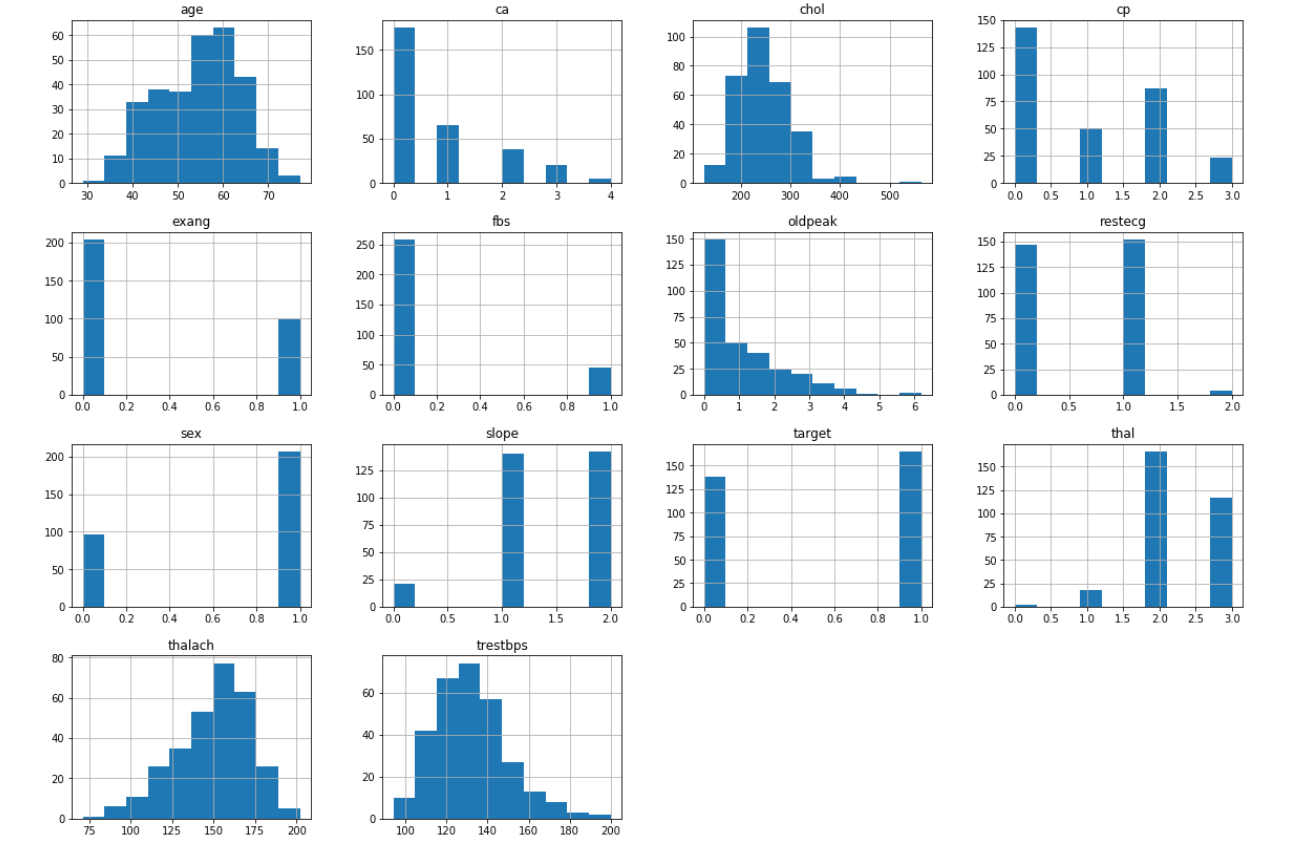
\includegraphics[scale=0.4]{images/hearthistogram.png}
    			\end{center}
	    		\begin{center}
	    			Figure 1.1 Histograms - Cleveland Heart Disease Dataset
	    		\end{center}
    \end{figure}
	
    \pagebreak
    The Count of each target class for the given dataset is as depicted below. The two target classes are:
    \begin{itemize}
    	\item 0: The instances that don’t have heart disease.
    	\item 1: The instances that have heart disease.
    \end{itemize}

	\begin{figure}
		\begin{center}
			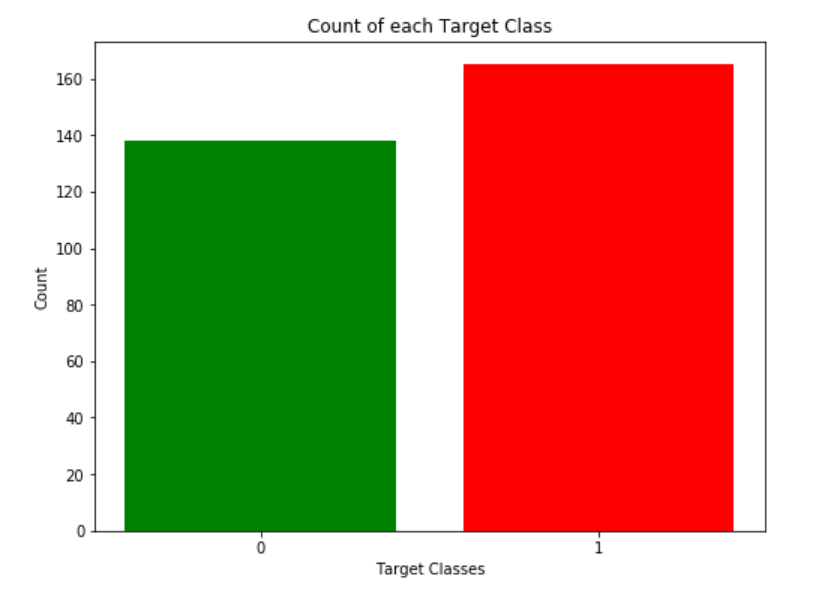
\includegraphics[scale=0.4]{images/heartcount.png}
		\end{center}
		\begin{center}
			Figure 1.2 Frequency Count of the Target Class
		\end{center}
	\end{figure}
	
	\subsubsection{Pima Indians Diabetes Dataset}
	
	This dataset\tiny\textcolor{white}{s}\normalsize is initially from the National Institute\tiny\textcolor{white}{s}\normalsize of Diabetes and Digestive\tiny\textcolor{white}{s}\normalsize and Kidney Disease. The goal\tiny\textcolor{white}{s}\normalsize of the dataset\tiny\textcolor{white}{s}\normalsize is to analytically foresee whether a patient has diabetes, in view of certain diagnostic estimations included in the dataset. The dataset comprises of $768$ individual clinical reports in which $500$ don't have any sickness. In this dataset all the patients are females of atleast $21$ years old of Pima Indian Heritage. 
	The dataset consists of $8$ features shown below:
	\begin{itemize}
		\item Pregnancies
		\item Glucose
		\item Blood Pressure 
		\item Skin Thickness
		\item Insuline
		\item BMI
		\item Diabetes Pedigree Function
		\item Age
	\end{itemize}
	The involvement of each attribute with respect to the number of instances are shown in Figure 1.3:
	\linebreak
	\begin{figure}	
		\begin{center}
			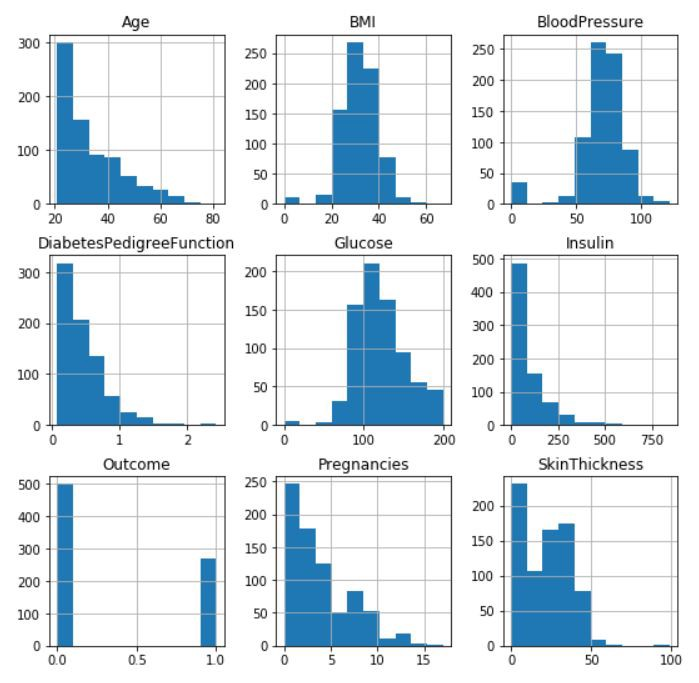
\includegraphics[scale=0.6]{images/diabeteshistogram.jpeg}
		\end{center}
	
		\begin{center}
			Figure 1.3 Histograms - Pima Indian Diabetes Dataset
		\end{center}
	\end{figure}
	\pagebreak
	The count of each target class for the given dataset is as depicted in Figure 1.4.
	\\
	The two target classes are:
	\begin{itemize}
		\item 0: The instances that don’t have diabetes.
		\item 1: The instances that have diabetes.
	\end{itemize}

	\begin{figure}	
		\begin{center}
			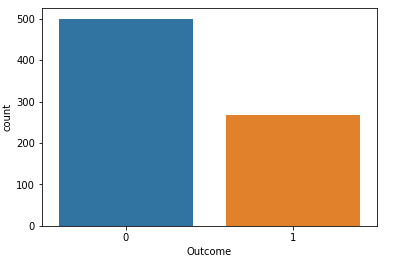
\includegraphics[scale=0.6]{images/diabetescount.png}
		\end{center}
		\begin{center}
			Figure 1.4 Frequency Count of the Target Class
		\end{center}
	\end{figure}
    
 
    
   \section{Summary of Gaps identified}
   Medical diagnosis is considered as a noteworthy yet unpredictable errand that should be done accurately and proficiently. The robotization of the equivalent would be exceptionally helpful. Clinical choice are frequently made dependent\tiny\textcolor{white}{s}\normalsize on doctor's instinct\tiny\textcolor{white}{s}\normalsize and experience\tiny\textcolor{white}{s}\normalsize as opposed to\tiny\textcolor{white}{o}\normalsize the knowledge\tiny\textcolor{white}{s}\normalsize of rich information covered up in the database\tiny\textcolor{white}{s}\normalsize. This training\tiny\textcolor{white}{s}\normalsize prompt undesirable inclinations, mistakes and extreme medical cost which influences the nature of administration\tiny\textcolor{white}{s}\normalsize gave to\tiny\textcolor{white}{o}\normalsize patients. Information mining can create an information-rich condition which can help to\tiny\textcolor{white}{o}\normalsize essentially improve the nature of\tiny\textcolor{white}{f}\normalsize clinical choices.
   
   
   
   	\section{Project problem statement and Objective}
   
   	\subsection{Problem Statement}
   	Doctor depends on common knowledge\tiny\textcolor{white}{s}\normalsize for treatment\tiny\textcolor{white}{s}\normalsize. When known facts is lacking, studies are recalled after some cases have been read again. But this method takes some time, where as if we use machine\tiny\textcolor{white}{s}\normalsize learning, the symptoms can be identified at early state\tiny\textcolor{white}{s}\normalsize.
   	For using machine\tiny\textcolor{white}{s}\normalsize learning\tiny\textcolor{white}{s}\normalsize, a huge amount of data is required. There is a very limited amount of data available depending on the\tiny\textcolor{white}{n}\normalsize disease\tiny\textcolor{white}{s}\normalsize. Also, the number\tiny\textcolor{white}{s}\normalsize of sample having 0 diseases is large when compared with number\tiny\textcolor{white}{s}\normalsize of\tiny\textcolor{white}{f}\normalsize samples with positive disease\tiny\textcolor{white}{s}\normalsize.
   	
   	\subsection{Objectives of the project}
   	\begin{enumerate}
   		\item The proposed system predicts heart diseases as well as the chances of diabetes.
   		\item Currently, there is no platform available which helps the users to predict the chances of heart disease and diabetes. We aim to build a powerful platform(web app) which helps the users to predict diabetes and heart disease.
   	\end{enumerate}
   
   
   	\section{Organization of the Report}
  	 The current chapter deals with the detailed Introduction of the project followed by the social and economical impacts of the project. The chapter also contains with the details of all the related research work carried out in this field.
  	 \\
  	 The organization of the remainder of the report is as per the following:
  	 \begin{itemize}
  	 	\item \textbf{Chapter 2}: This section contains the high-level structure of the proposed model alongside the software development methodologies utilized by the project developers during the advancement of this undertaking.
  	 	\item \textbf{Chapter 3}: This chapter contains the design details and UML diagrams of the model along with the data structures and algorithms used in this project.
  	 	\item \textbf{Chapter 4}: This chapter includes the implementation level information of the aforementioned project.
  	 	\item \textbf{Chapter 5}: The testing details of the final model is included in this chapter.
  	 	\item \textbf{Chapter 6}: This part of the report contains the final conclusion drawn along with the future scope of this project.
  	 	\
  	 	\tiny\textcolor{white}{\textbf{Chapter 4}: This chapter includes the implementation level information of the aforementioned project.}\normalsize
  	 	\tiny\textcolor{white}{\item \textbf{Chapter 5}: The testing details of the final model is included in this chapter.}\normalsize
  	 	\tiny\textcolor{white}{\textbf{Chapter 6}: This part of the report contains the final conclusion drawn along with the future scope of this project.}\normalsize
  	 \end{itemize}
    
     \chapter{High-level Design}
    
   	This chapter\tiny\textcolor{white}{s}\normalsize covers the engineering modules on which this project\tiny\textcolor{white}{s}\normalsize is build. First, we briefly define the\tiny\textcolor{white}{se}\normalsize incremental model\tiny\textcolor{white}{s}\normalsize, which includes several cycles after which the current version of the web app has been obtained. Then, there is the definition of agility that means regular status check of the project by the faculty panel and the project guide. We then briefly describe the Scrum, namely the regular meetings that we had with the team members.
    \section{Software Development Methodology}
    	Software Development Life Cycle (SDLC) is a technique for setting up, creating and testing available programming from merchants (as in Figure 2.1). Sending better programming from the SDLC means that the client meets or exceeds the client's expectations. SDL is a technology used for a product's project, a product's association. This includes creating, maintaining, abusing, and improving programming features. The figure below is a graphic example of the various stages of a typical SDLC.
    	
    	\begin{figure}
    		\begin{center}
    			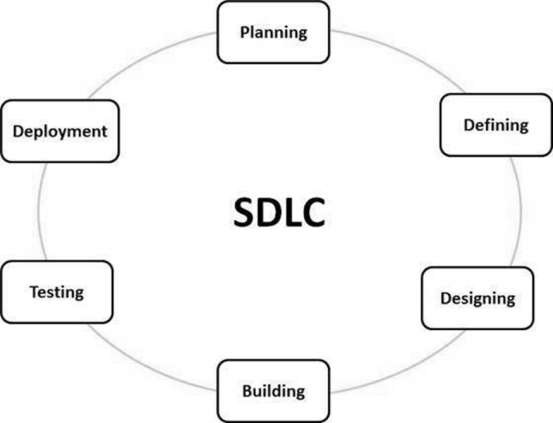
\includegraphics[scale=0.8]{images/sdlc.png}
    		\end{center}
    		
    		
    		\begin{center}
    			Figure 2.1 Software Development Life Cycle
    		\end{center}
    	\end{figure}
    
    	\paragraph{}
    	The detailed SDLC outline (Figure 2.1) shows how all the steps have been contributed to make the proposed work accurate and precise.
    	A typical software development lifecycle consists of the following steps:
    	
    	 \subsection{Stage 1: Planning and Requirement Analysis}
    	The simulation test is the most important and central stage in the SDLC. This is done by the elderly people in the group with significant participation from clients, business offices, advertising studies, space\tiny\textcolor{white}{s}\normalsize specialist in this business. This data was later used to adjust the required operational procedures and to keep the devil's ability to understand effective, operational and specific zones. The process of standardized certification requirements is tailored to the curriculum and evidence of risk-related risks similar to that in the Master Mining stage. The result considers the outcome of a very specific decision to describe important specific ways of insight, which can be done after a minute's careful understanding of the task.
    	
    	\subsection{Stage 2: Defining Requirements}
    	Once the required test is completed the stage will then be able to image and report the needs of the product and get help from customers or marketing agents. This is done through an SSR (Software Requirements Explanation) report, which contains the essentials to be had and is created during the life cycle.
    	
    	\subsection{Stage 3: Designing the Product Architecture}
    	A systematic approach clearly defines all the plan modules of the item accordingly with the appearance of the data flow and the external and non-modular models (to expect one). Within the framework of the significant number of proposed design models, the unconditional components in the DDS must be minimized.
    	
    	\subsection{Stage 4: Building or Developing the Product}
    	Real change begins in this period\tiny\textcolor{white}{s}\normalsize of SDLC, and things are made. DDS generates programming code during these stage\tiny\textcolor{white}{s}\normalsize. If the arrangement is done in a positive way, the code can be a long life problem. The developers should go after their representation of these code rules and use their affiliation and programming gadgets such as code compilers, middlemen, checker debuggers, etc. to generate the code. Separate state-of-the-art programming programmers for coding, for example C, C ++, Pascal\tiny\textcolor{white}{s}\normalsize, Java, and Python are used. The programming language is used to select the type of computer programs to write.
    	
    	\subsection{Stage 5: Testing the Product}
    	This stage is usually a part of a wider number of stages, as in the front-line SDLC model, testing processes are generally two-connected with each period of the SDLC. However, this phase checks that the bus, after representing something, has grown, settled and re-examined, until it meets the quality measures shown in the SRS.

    	\subsection{Stage 6: Deployment in the Market and Maintenance}
    	 Once this item is tried and arranged to pass it is regularly issued in the right market. The remodeling now and again begins in phases, as evidenced by this affiliate business strategy. The first thing may be issued in a limited area and tried in a valid business state (UAT-User affirmation testing) then in view of the information, the item can be released as it is or parcel of promotion. With the proposed changes to focus on. After releasing the item into the market, its upbringing has improved the condition of existing customers.
    	
    	\section{Architecture}
    	
    	\begin{figure}
    		\begin{center}
    			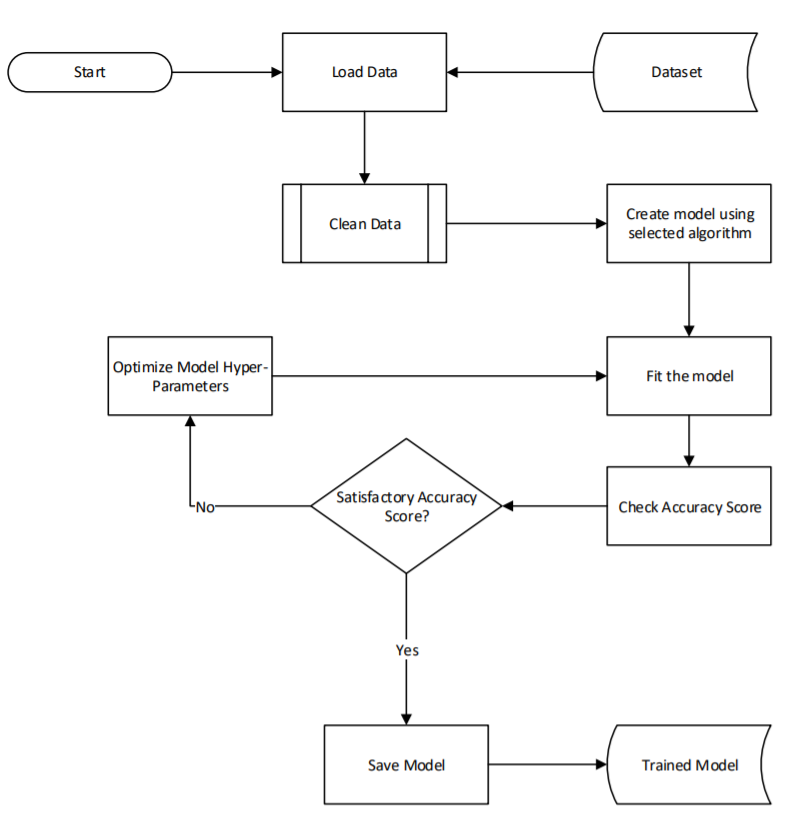
\includegraphics[]{images/df.png}
    		\end{center}
    		
    		\begin{center}
				Figure 2.2: Initial design of the proposed system
    		\end{center}
    	\end{figure}
    	
    	
    	This report will provide a result that is distributed into three phases:
    
    	\begin{enumerate}
    		\item \textbf{Analysis Phase (Based on the Dataset): } At this stage, the main concentration is to examine the information from the data set and to illuminate the patient's medical data. At this stage, we try to analyze which medical data or medical values have the greatest impact on disease prognosis and which features have the least impact.
    	\item \textbf{Combining analysis stage with the parameters:} At this stage, we give some conditions based on the patient's condition (whether the patient is suffering from heart disease and diabetes). The application applies various machine learning algorithms to generate a module, which in turn is used in the prediction process.  
    	\item \textbf{Prediction Phase:} At this stage, we disclose the results and declare the possibility that the person is suffering from heart disease or diabetes. The results were predicted using different machine learning algorithms from user-defined values.
    	\end{enumerate}
    	
    	\section{Incremental Model}
    	
    	The\tiny\textcolor{white}{n}\normalsize incremental frames represent a strategy for\tiny\textcolor{white}{m}\normalsize programming movement where something is designed, processed and maximized (until some degree more solid each time) until the task is completed. 2.2). It both turns and comes back down. Things get caught up when he caters to the more prominent part of his needs. This indicates that the datasets of the waterfall appeared on a civilizational basis of the prototype. The item is delivered in separate sections, each of which is organized and structured in an anonymized way (together with the name). Each part is sent to the client when it is completed. This serprise avoids the use of products and maintains a strategic space from long growth times. It likewise guarantees the removal of an important starting capital and the shortage period. This shows that growth spurt is at the same time promoting the frightening effects of modern systems at the same time.
    	\paragraph{}
    	Characteristics of\tiny\textcolor{white}{f}\normalsize the Incremental\tiny\textcolor{white}{s}\normalsize Model:
    	\begin{itemize}
    		\item Systems are isolated into different small units.
    		\item Partial system are meant to deliver the ultimate framework.
    		\item Firstly the required procedures are performed.
    		\item What is required is cemented when an extended bit is produced.
    	\end{itemize}
    	
    	
    	\begin{figure}
    		\begin{center}
    			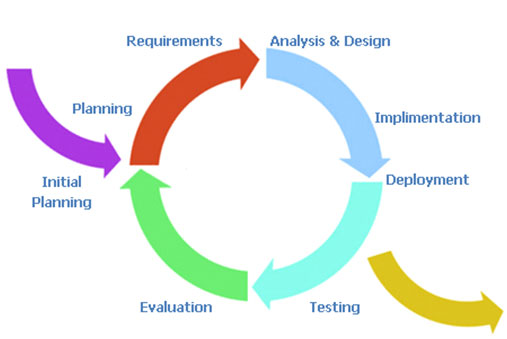
\includegraphics[]{images/cycle.jpg}
    		\end{center}
    		
    		
    		\begin{center}
    			Figure 2.3: Incremental model\tiny\textcolor{white}{s}\normalsize for project
    		\end{center}
    	\end{figure}
    	After each cycle, backward testing is facilitated. In the midst of this test, the damaging parts of the product can be seen lightly so that some changes can be made internally at any one stress. It is, in general, easy to examine and explain the different approaches to the programming movement\tiny\textcolor{white}{s}\normalsize in light\tiny\textcolor{white}{s}\normalsize of\tiny\textcolor{white}{f}\normalsize the ways in which the eight-part changes are made today between each section. It focuses more on the center and takes the internal scrutiny of each section seriously. The customer seems to respond to highlighting and evaluating the product being used for any desired changes. The essential thing is the faster and lower cost of the accelerator model.
    	
    	\section{Agility and Scrum}
    	Advanced programming can be a strategy for creating programming techniques (such as another programming reverse systems - waterfall model, V-model, incremental shows etc.). In English, detectors mean the ability to move quickly and easily, and reacting quickly is often an important piece of well-structured programming reversals.
    	In traditional expert programming such as Waterfalls model, an outage can take several months and a long time because the client may not get the opportunity to see the end result of that commitment. In the exceptional case, the non-Agile assignments determine the timeframe for submission, arrangement, development, testing and client acceptance testing failures, spray work done sprints or attributes that are in term today (sprint) / Squares can move from 2 weeks to 2 months) in the midst of selected skills.
    	
    	\subsection{Agility and the cost of change}
    	The general method of\tiny\textcolor{white}{f}\normalsize undertaking in programming movement is the advance increment nonlinearly as\tiny\textcolor{white}{s}\normalsize an endeavour advances (Figure 2.3). It is fairly fundamental to oblige and adjust when a\tiny\textcolor{white}{n}\normalsize thing\tiny\textcolor{white}{s}\normalsize pack\tiny\textcolor{white}{s}\normalsize is gathering essentials (exactly on time in a meander). A pre-owned circumstance must be changed, the rundown of the breaking point likely could be broadened, or made express could be changed. The expense of achieving this work is unimportant, and the exertion required won't ominously influence the outcome of the undertaking. Nevertheless, envision a condition where we fast forward different months. The group is amidst support testing (something that happens commonly late inside the wander), and a basic partner is requesting an essential reasonable change. The modify requires a change to the compositional organize of the thing, the diagram and movement of three present-day parts, alterations to another five segments, the game plan of unused tests, and so on.
    	
    	
    	\begin{figure}
    		\begin{center}
    			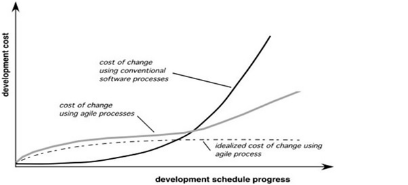
\includegraphics[scale=0.7]{images/chotu.png}
    		\end{center}
    		
    		
    		\begin{center}
    				Figure 2.4: Agility and the cost of change
    		\end{center}
    	\end{figure}

    	\paragraph{}
    	\textbf{Advantages of Agile Methodology:}
    	\begin{itemize}
    		\item In Dexterous framework the advancement\tiny\textcolor{white}{s}\normalsize of\tiny\textcolor{white}{f}\normalsize making PC program is unremitting. 
    		\item The clients are fulfilled considering reality that after each Sprint, the working fragment of the thing is given to them.
    		\item Clients can see the working part which fulfilled their needs. 
    		\item in the event that the customers have any analysis or any change inside the bit by then it tends to be obliged inside the show area of the thing. 
    		\item In Spry framework, the bit by bit affiliations are required between the bosses and the creators. 
    		\item In this structure thought is paid to the extraordinary chart of the thing.
    	\end{itemize}
    	
    	
    	
    	\section{Scrum}
    	Scrum could be a fast structure for sorting out work with an element on programming improvement. It is sorted out gatherings of three to nine fashioners who break their work into works out that should be conceivable inside time-boxed cycles, called runs (routinely fourteen days) and track advance and re-graph in 15-minute stand-up social undertakings, called a tiny bit at a time scrums. Ways to deal with manage sifting through made by contrasting scrum packages in progressively basic affiliations concrete Large-Scale Scrum, Scaled Dexterous System (SAF) and Scrum of Scrums, among others.
    	
    	\subsection{Activities performed by the team in the scrum}
    	\begin{itemize}
    		\item At the initial stages, extension and plan of the project are chosen. 
    		\item Regular commitment on a week by week premise to keep a mind all the exercises are in a state of harmony with one another. 		
    		\item Engagement with the project guide assisted with doing the necessary adjustment of the project.    		
    		\item Requirement gathering was done in a gradual manner.     		
    		\item project was separated into various components with the goal that legitimate appropriation of work should be possible in the group. 
    		\item Each colleague is answerable for its doled out work.    		
    		\item Every 14 days progress was checked and new objectives of the project were characterized to concentrate on.    		
    		\item After the development of each module testing was done to ensure the best possible working of the module.    		
    		\item All the components were coordinated to ensure everything functions admirably together.    		
    		\item Report composing was done on a nonstop premise to catch all the outcomes and conversations.
    	\end{itemize}
    	
    	
    	\begin{figure}
    		\begin{center}
    			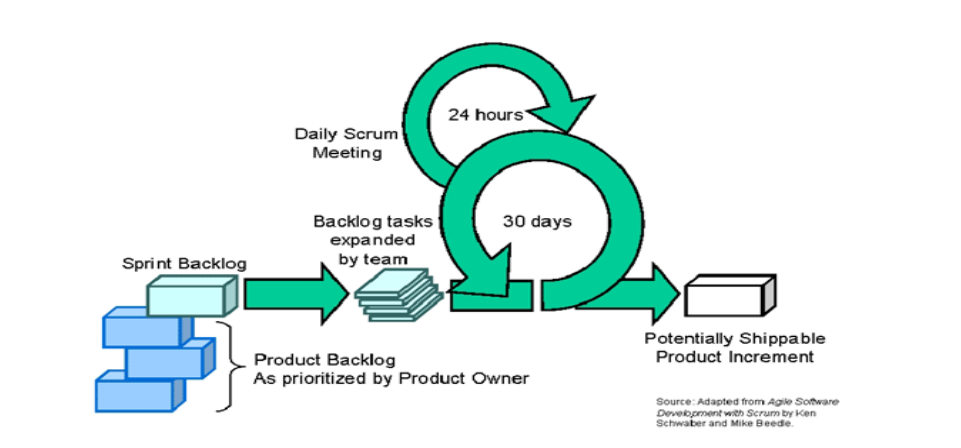
\includegraphics[scale=0.5]{images/animesh_chotu.png}
    		\end{center}
    		
    		\begin{center}
    			Figure 2.5: Scrum design of the project
    		\end{center}
    	\end{figure}
		\paragraph{}
    	Scrum consist of three roles: Product Owner, Scrum Master, and Team:
    	\begin{itemize}
    		\item \textbf{Item Owner:} The Item Owner ought to be cautious with exchange with vision, star, and responsiveness. The Item Proprietor is at risk for perseveringly giving the vision and necessities to the change gathering. It's every so often hard for Product Proprietors to strike the most ideal difference in thought. Since Scrum respects self-relationship among get-togethers, an Item Proprietor must battle the need. to humbler scale direct. Meanwhile, Item Proprietors must be available to answer ask from the get-together.
    		
    		\item \textbf{Scrum Master:} The Scrum Master\tiny\textcolor{white}{s}\normalsize goes round as helper\tiny\textcolor{white}{s}\normalsize for the Item\tiny\textcolor{white}{s}\normalsize Proprietor and the social gathering. The Scrum Ace doesn't deal with the social event. The Scrum Ace attempts to rinse any obstructions that are blocking the social issue\tiny\textcolor{white}{s}\normalsize from satisfying its run goals. This secures in the social event to stay innovative and valuable while ensuring its triumphs are obvious to the Item Proprietor.
    		
    		\item \textbf{Team:} As showed up by Scrum's facilitator, "the social occasion is absolutely self-managing." The progression hard and fast is fit for self-sorting out to signify work. A Scrum advancement store up contains around seven completely dedicated individuals (authoritatively 3-9), preferably in one social event room ensured from outside redirections. For programming meanders, a standard social affair solidifies a blend of programming engineers, modelers, programming engineers, auditors, QA experts, analysers, and UI organizers.
    	\end{itemize}
    	
    	
    	\section{Functional Requirements}
    	\begin{itemize}
    		\item Predict the probability of Heart Disease and Diabetes with given user inputs.
    		\item Contribute to the dataset or request to add functionalities.
    	\end{itemize}
    
    	
    	\section{Non-Functional Requirement}
    	\paragraph{}
    	Non-rational necessities are prerequisites that exhibit rules that can be utilized to pass judgment on the activity of a structure, as opposed to explicit practices. This could be showed up particularly in association with important prerequisites that portray explicit direct or cutoff points. 
    	\paragraph{} 
    	Non-practical necessities are a noteworthy piece of the time called characteristics of a structure. Unmistakable verbalizations for utilitarian necessities are restrictions, quality attributes, quality targets, nature of association prerequisites and nonbehavioral fundamentals.
    	
    	\section{Feasibility Analysis}
    	\subsection{Technical feasibility} 
    	The project is technically feasible as it very well may be manufactured utilizing the currently accessible advances. It is an electronic application that utilizes the Grails Framework. The innovation required by Disease Predictor is accessible and consequently, it is technically feasible.
    	
    	\subsection{Economic feasibility} 
    	The project is economically feasible as the cost of the project is included uniquely in the deployment of the web-app. As the information tests expands, which devour additional time and handling power. All things considered, a superior processor may be required.
    	\tiny\textcolor{white}{ As the information tests expands, which devour additional time and handling power. All things considered, a superior processor may be required. As the information tests expands, which devour additional time and handling power. All things considered, a superior processor may be required. As the information tests expands, which devour additional time and handling power. All things considered, a superior processor may be required. As the information tests expands, which devour additional time and handling power. All things considered, a superior processor may be required. As the information tests expands, which devour additional time and handling power. All things considered, a superior processor may be required. As the information tests expands, which devour additional time and handling power. All things considered, a superior processor may be required. As the information tests expands, which devour additional time and handling power. All things considered, a superior processor may be required. As the information tests expands, which devour additional time and handling power. All things considered, a superior processor may be required. As the information tests expands, which devour additional time and handling power. All things considered, a superior processor may be required. As the information tests expands, which devour additional time and handling power. All things considered, a superior processor may be required. As the information tests expands, which devour additional time and handling power. All things considered, a superior processor may be required. As the information tests expands, which devour additional time and handling power. All things considered, a superior processor may be required. As the information tests expands, which devour additional time and handling power. All things considered, a superior processor may be required. As the information tests expands, which devour additional time and handling power. All things considered, a superior processor may be required. As the information tests expands, which devour additional time and handling power. All things considered, a superior processor may be required. As the information tests expands, which devour additional time and handling power. All things considered, a superior processor may be required. As the information tests expands, which devour additional time and handling power. All things considered, a superior processor may be required. As the information tests expands, which devour additional time and handling power. All things considered, a superior processor may be required. As the information tests expands, which devour additional time and handling power. All things considered, a superior processor may be required. As the information tests expands, which devour additional time and handling power. All things considered, a superior processor may be required. As the information tests expands, which devour additional time and handling power. All things considered, a superior processor may be required. As the information tests expands, which devour additional time and handling power. All things considered, a superior processor may be required. As the information tests expands, which devour additional time and handling power. All things considered, a superior processor may be required. As the information tests expands, which devour additional time and handling power. All things considered, a superior processor may be required.}\normalsize
	
	\chapter{Detailed Design}
    	This section will cover the plan of our model in detail. Right off the bat with an interface plan that will give a nitty gritty clarification about the interface plan, and afterward with the Data Structure and Algorithms that have been utilized in the project. The entire point by point system plan with use case has been appeared in Fig 3.1.
    	
    	\section{Interface Design}
    	This section depicts the client's connection with the interface. The between face plans/screen-shots have been included a request to give a superior perspective on the user interface.
    	
    	
    		\begin{center}
    			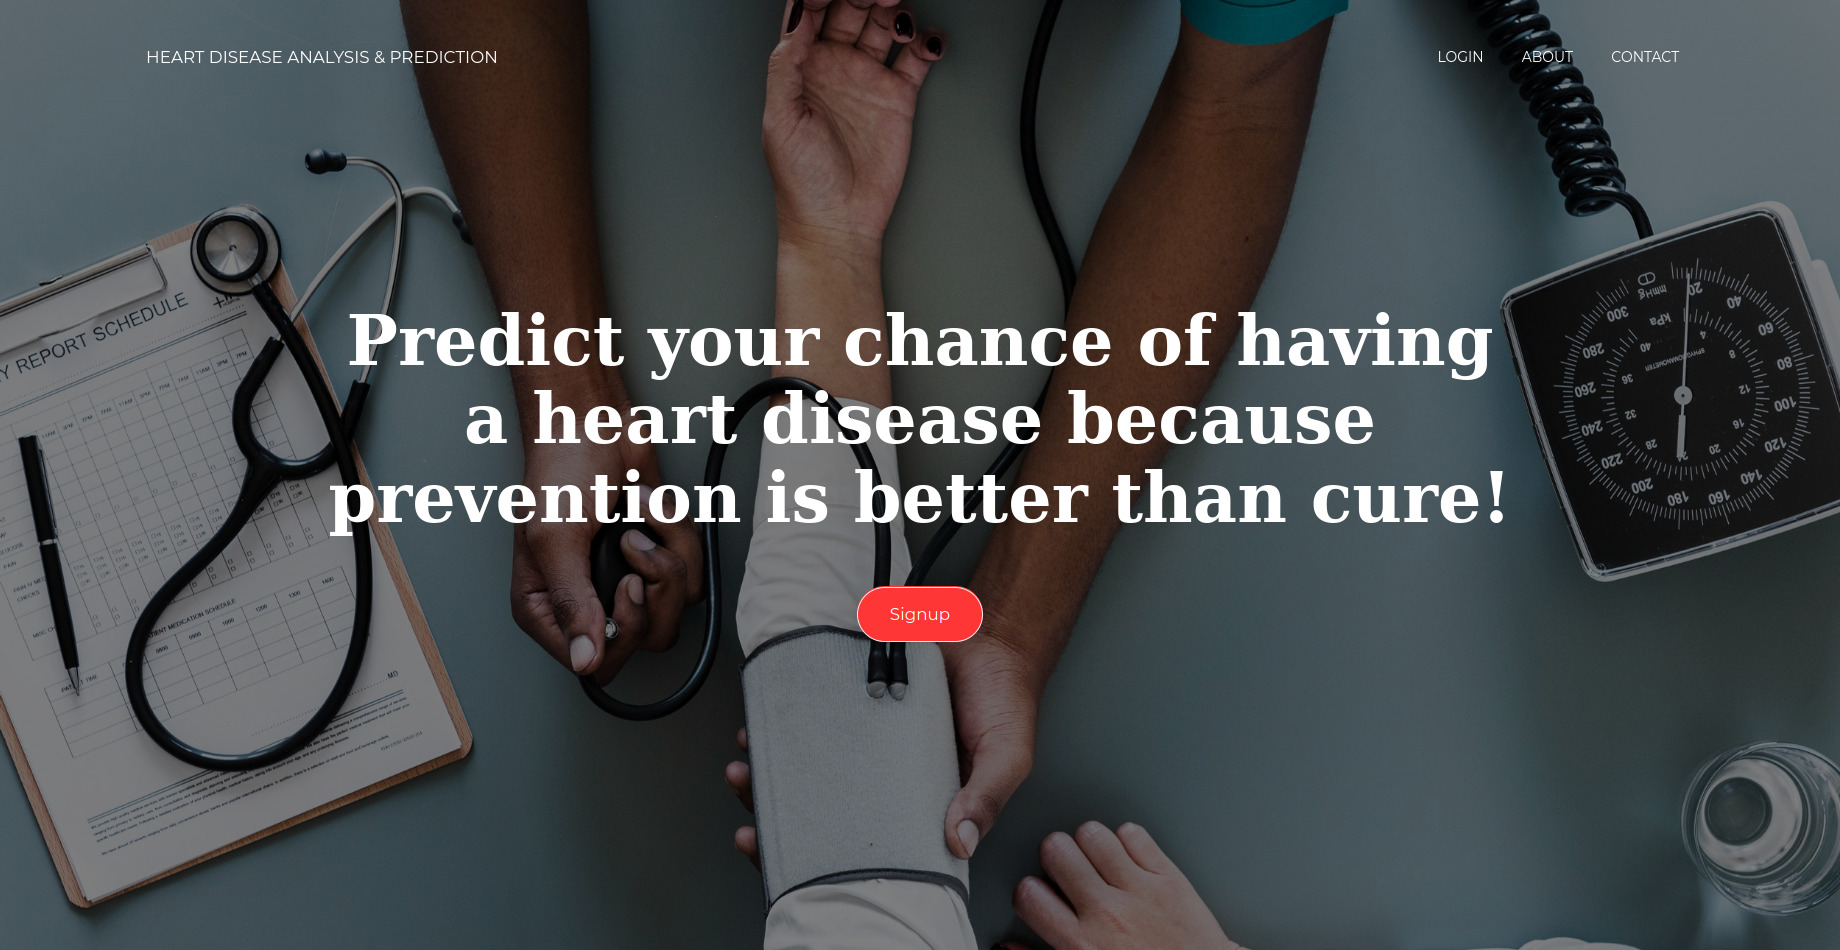
\includegraphics[width=17cm]{Screenshots/home1.jpg}
    			\begin{figure}
    				\caption{Home page }
    			\end{figure}
    		\end{center}
    		
    		\begin{figure}
    				\begin{center}
    				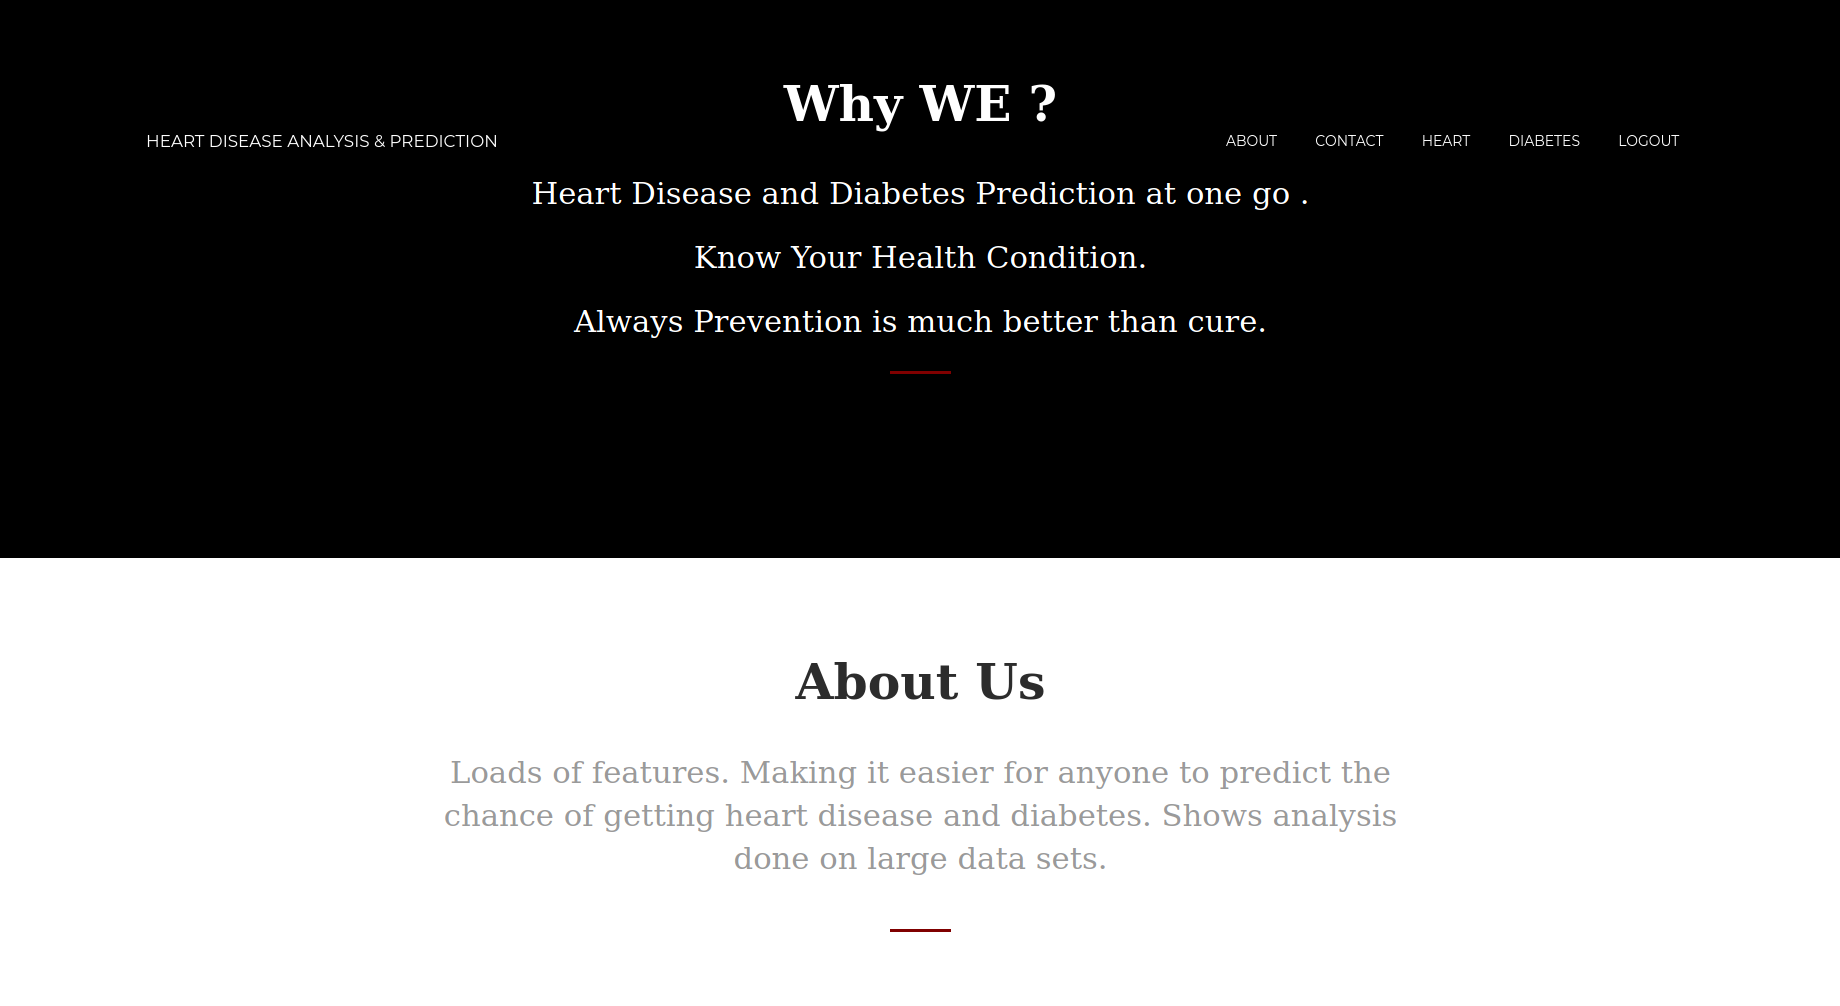
\includegraphics[width=17cm]{Screenshots/home2.PNG}
    				\caption{Home}
    				\end{center}
    		\end{figure}
    		
    		\begin{figure}
    				\begin{center}
    				
\includegraphics[width=10cm,scale=0.5]{Screenshots/home3.PNG}
    				\caption{Home}
    				\end{center}
    		\end{figure}
    
    			\begin{figure}
    				\begin{center}
    				
\includegraphics[width=17cm]{Screenshots/sign-up.jpg}
    				
\includegraphics[width=17cm]{Screenshots/login.PNG}
    				\caption{SignUp and Login feature}
    				\end{center}
    			\end{figure}
    			
    			\begin{figure}
    				\begin{center}
    				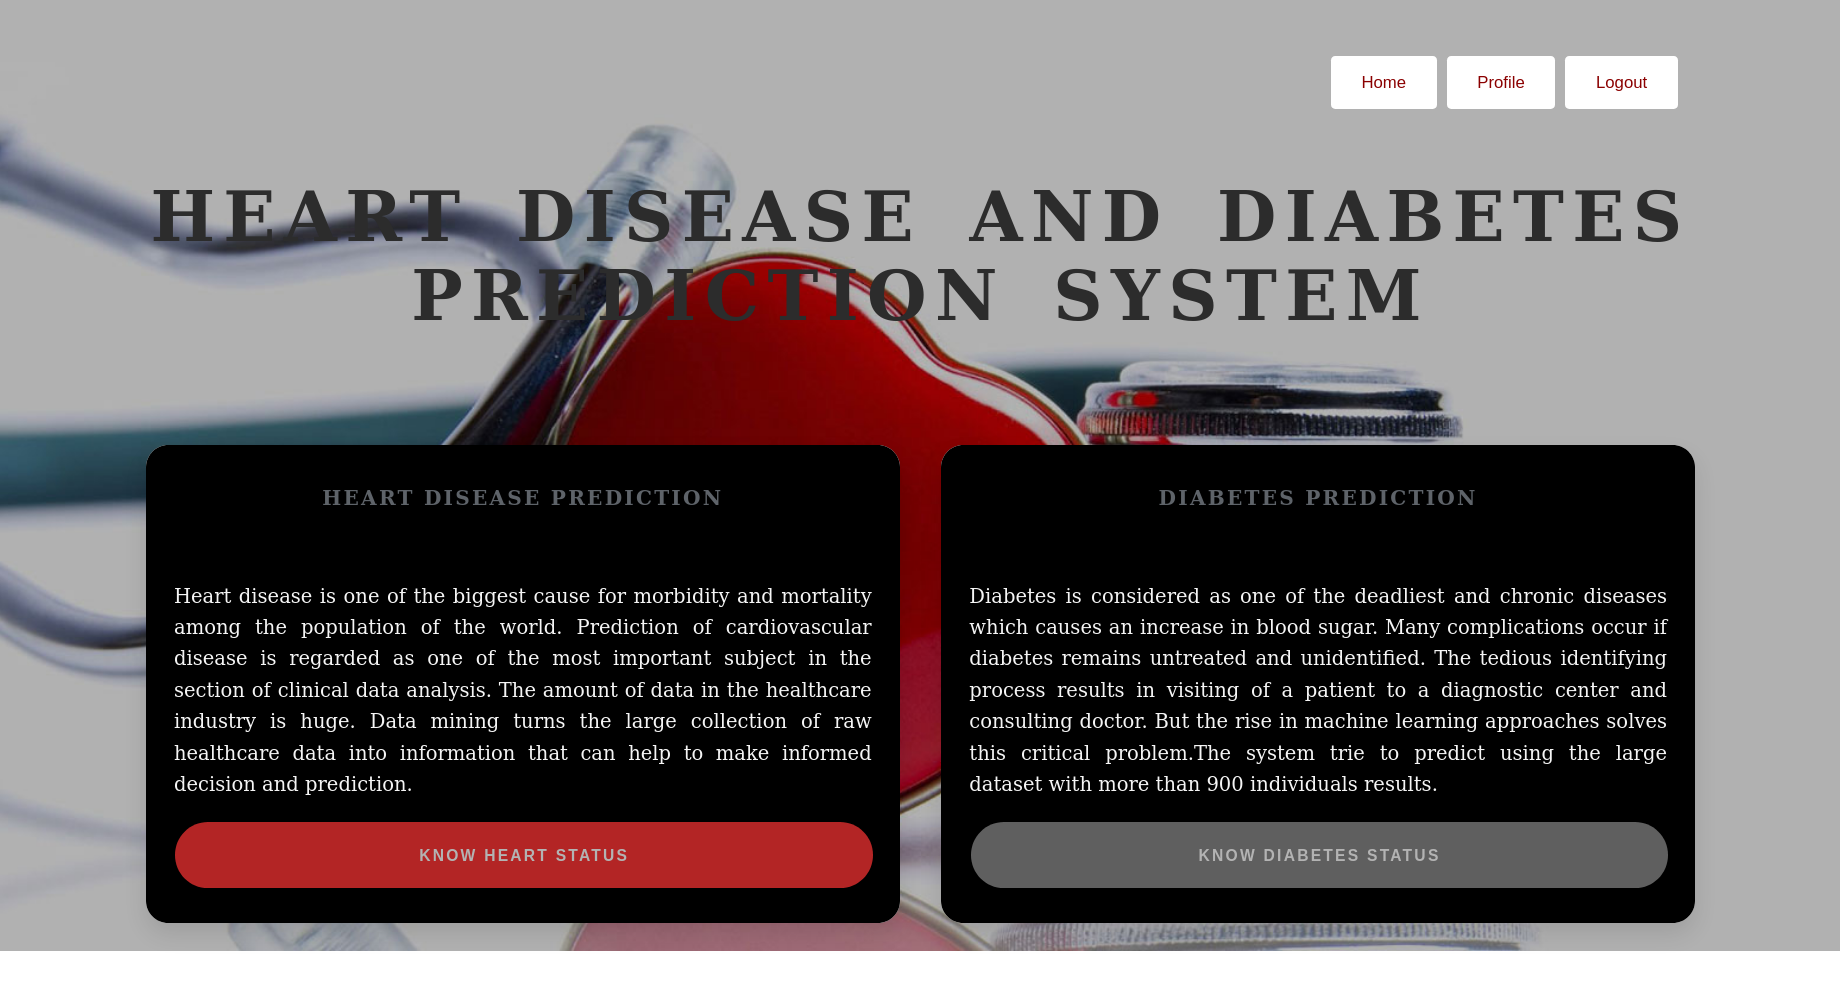
\includegraphics[width=17cm]{Screenshots/description-predict.PNG}
    				\caption{options of Prediction Engine}
    				\end{center}
    			\end{figure}
    			
    			\begin{figure}
    				\begin{center}
    				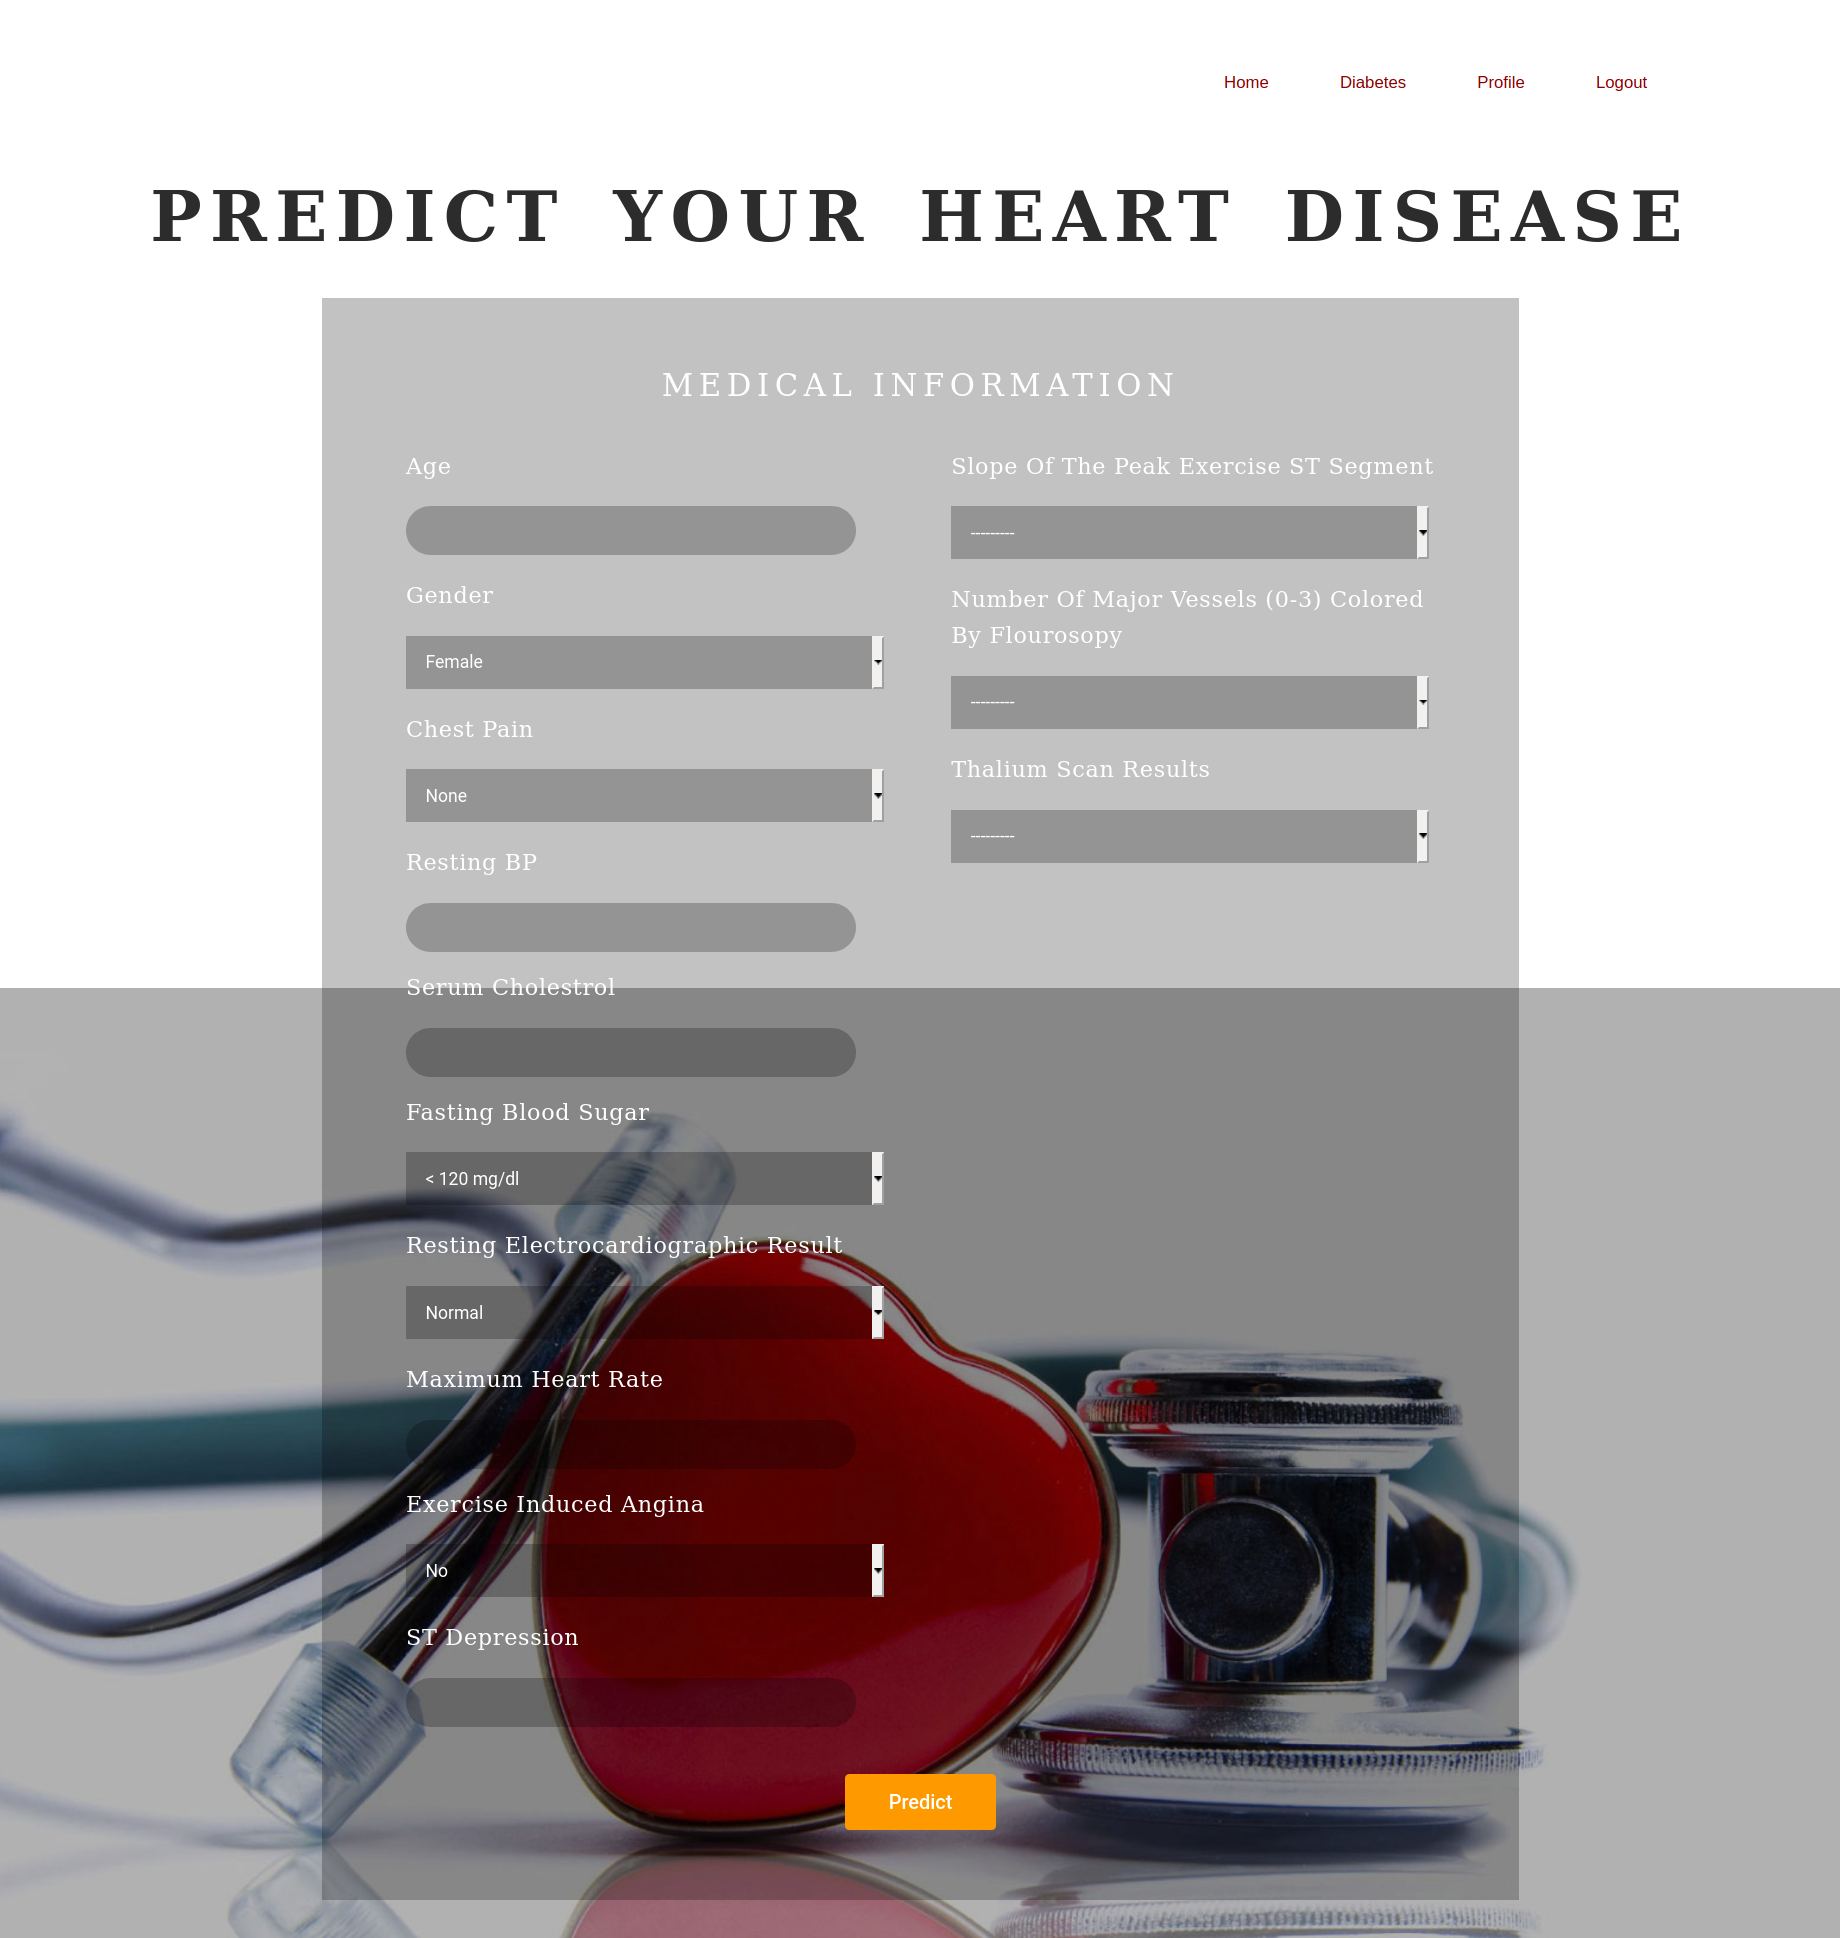
\includegraphics[width=17cm]{Screenshots/heart-form.PNG}
    				\caption{Heart diseases prediction form for patient}
    				\end{center}
    			\end{figure}
    			
    			\begin{figure}
    				\begin{center}
    				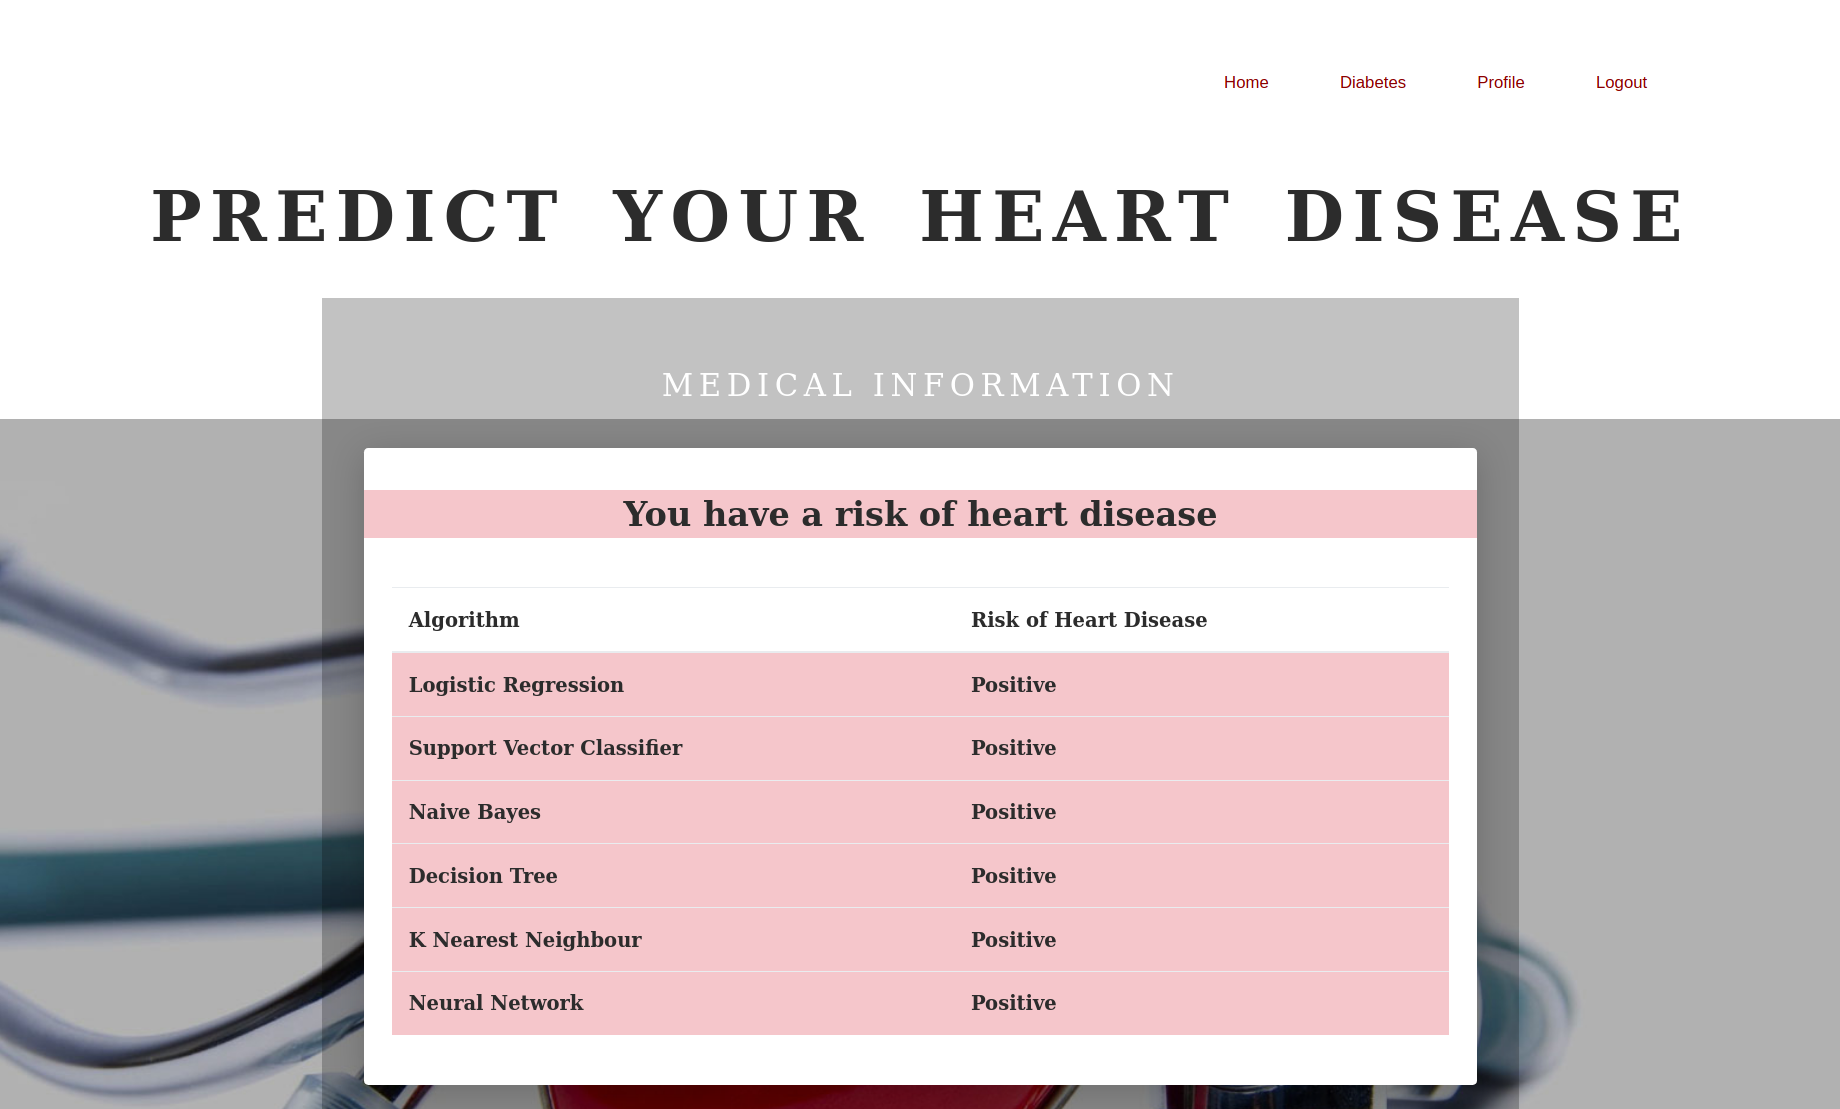
\includegraphics[width=17cm]{Screenshots/heart-result.PNG}
    				\caption{Heart diseases prediction result for patient}
    				\end{center}
    			\end{figure}
    			
    			\begin{figure}
    				\begin{center}
    				
\includegraphics[width=17cm]{Screenshots/diabetes-form.PNG}
    				\caption{Diabetes prediction form for patient}
    				\end{center}
    			\end{figure}
    			
    			\begin{figure}
    				\begin{center}
    				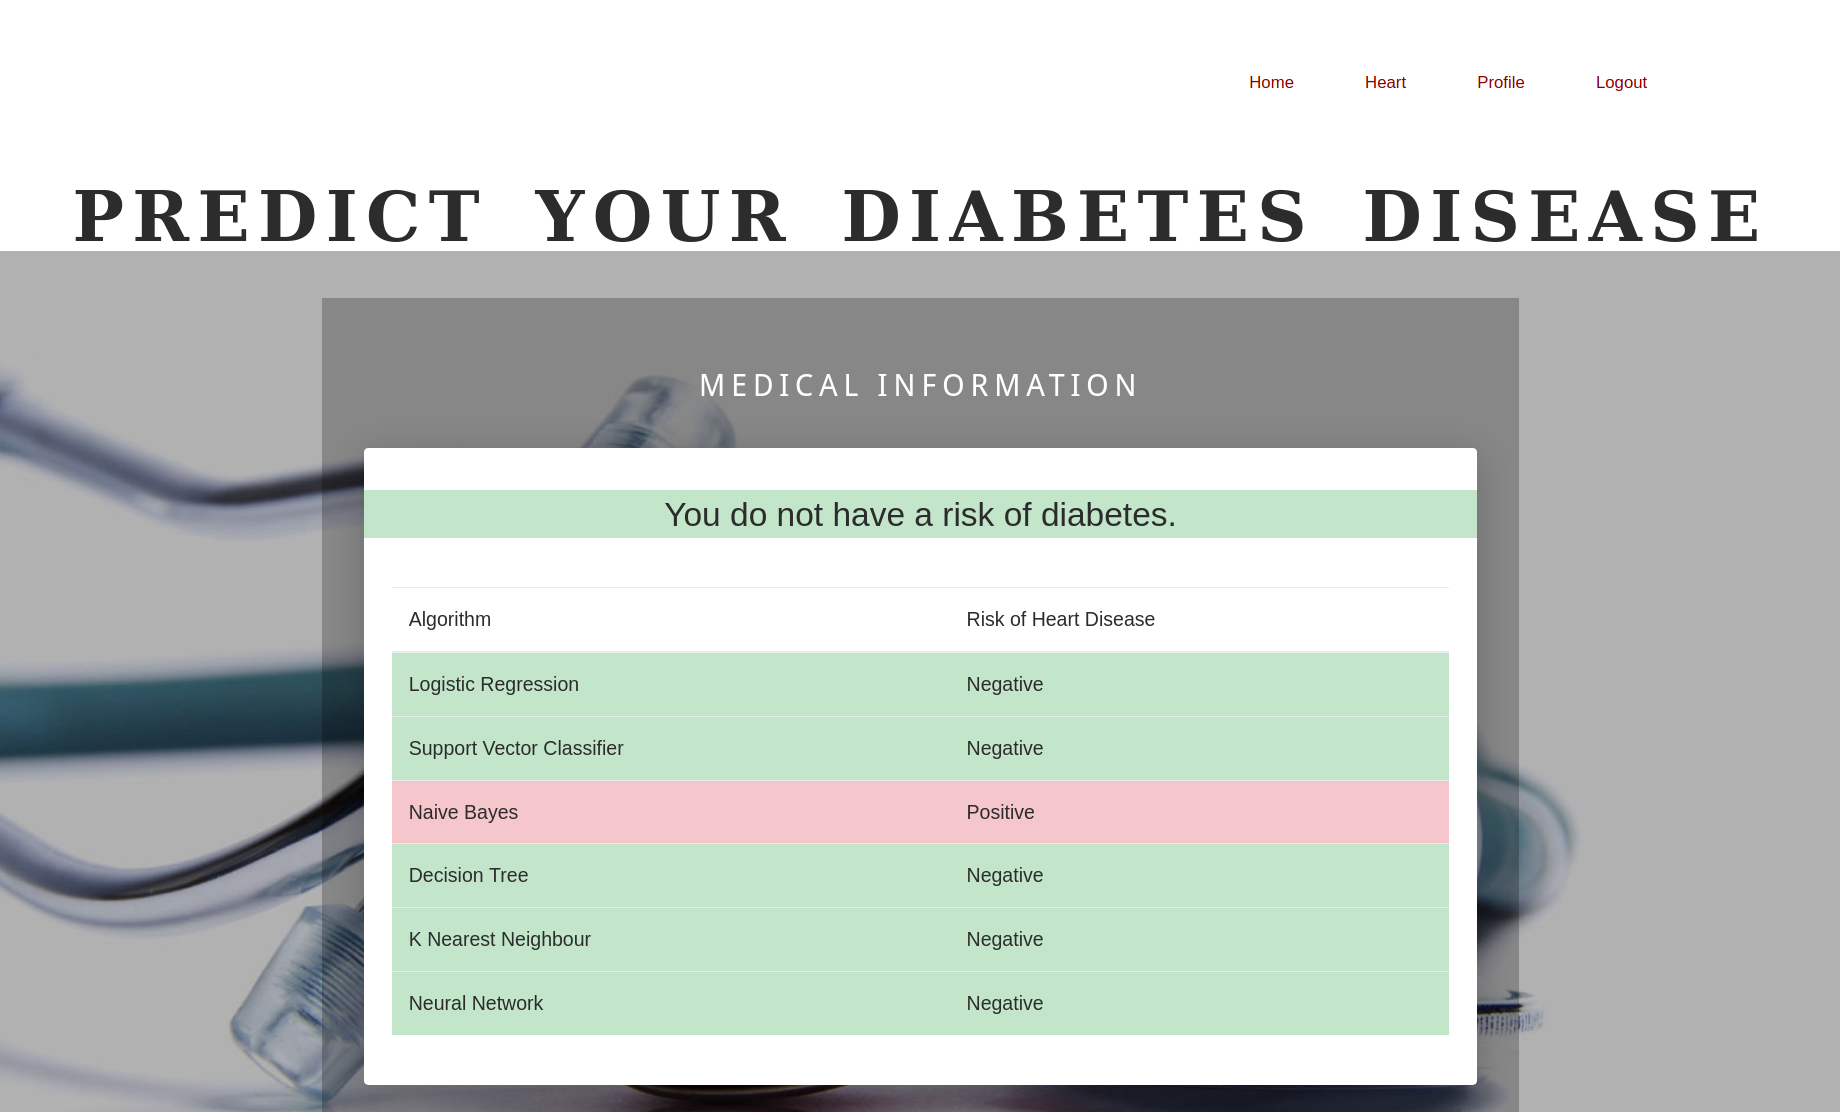
\includegraphics[width=17cm]{Screenshots/diabetes-result.PNG}
    				\caption{Diabetes prediction result for patient}
    				\end{center}
    			\end{figure}
    			
    			\begin{figure}
    				\begin{center}
    				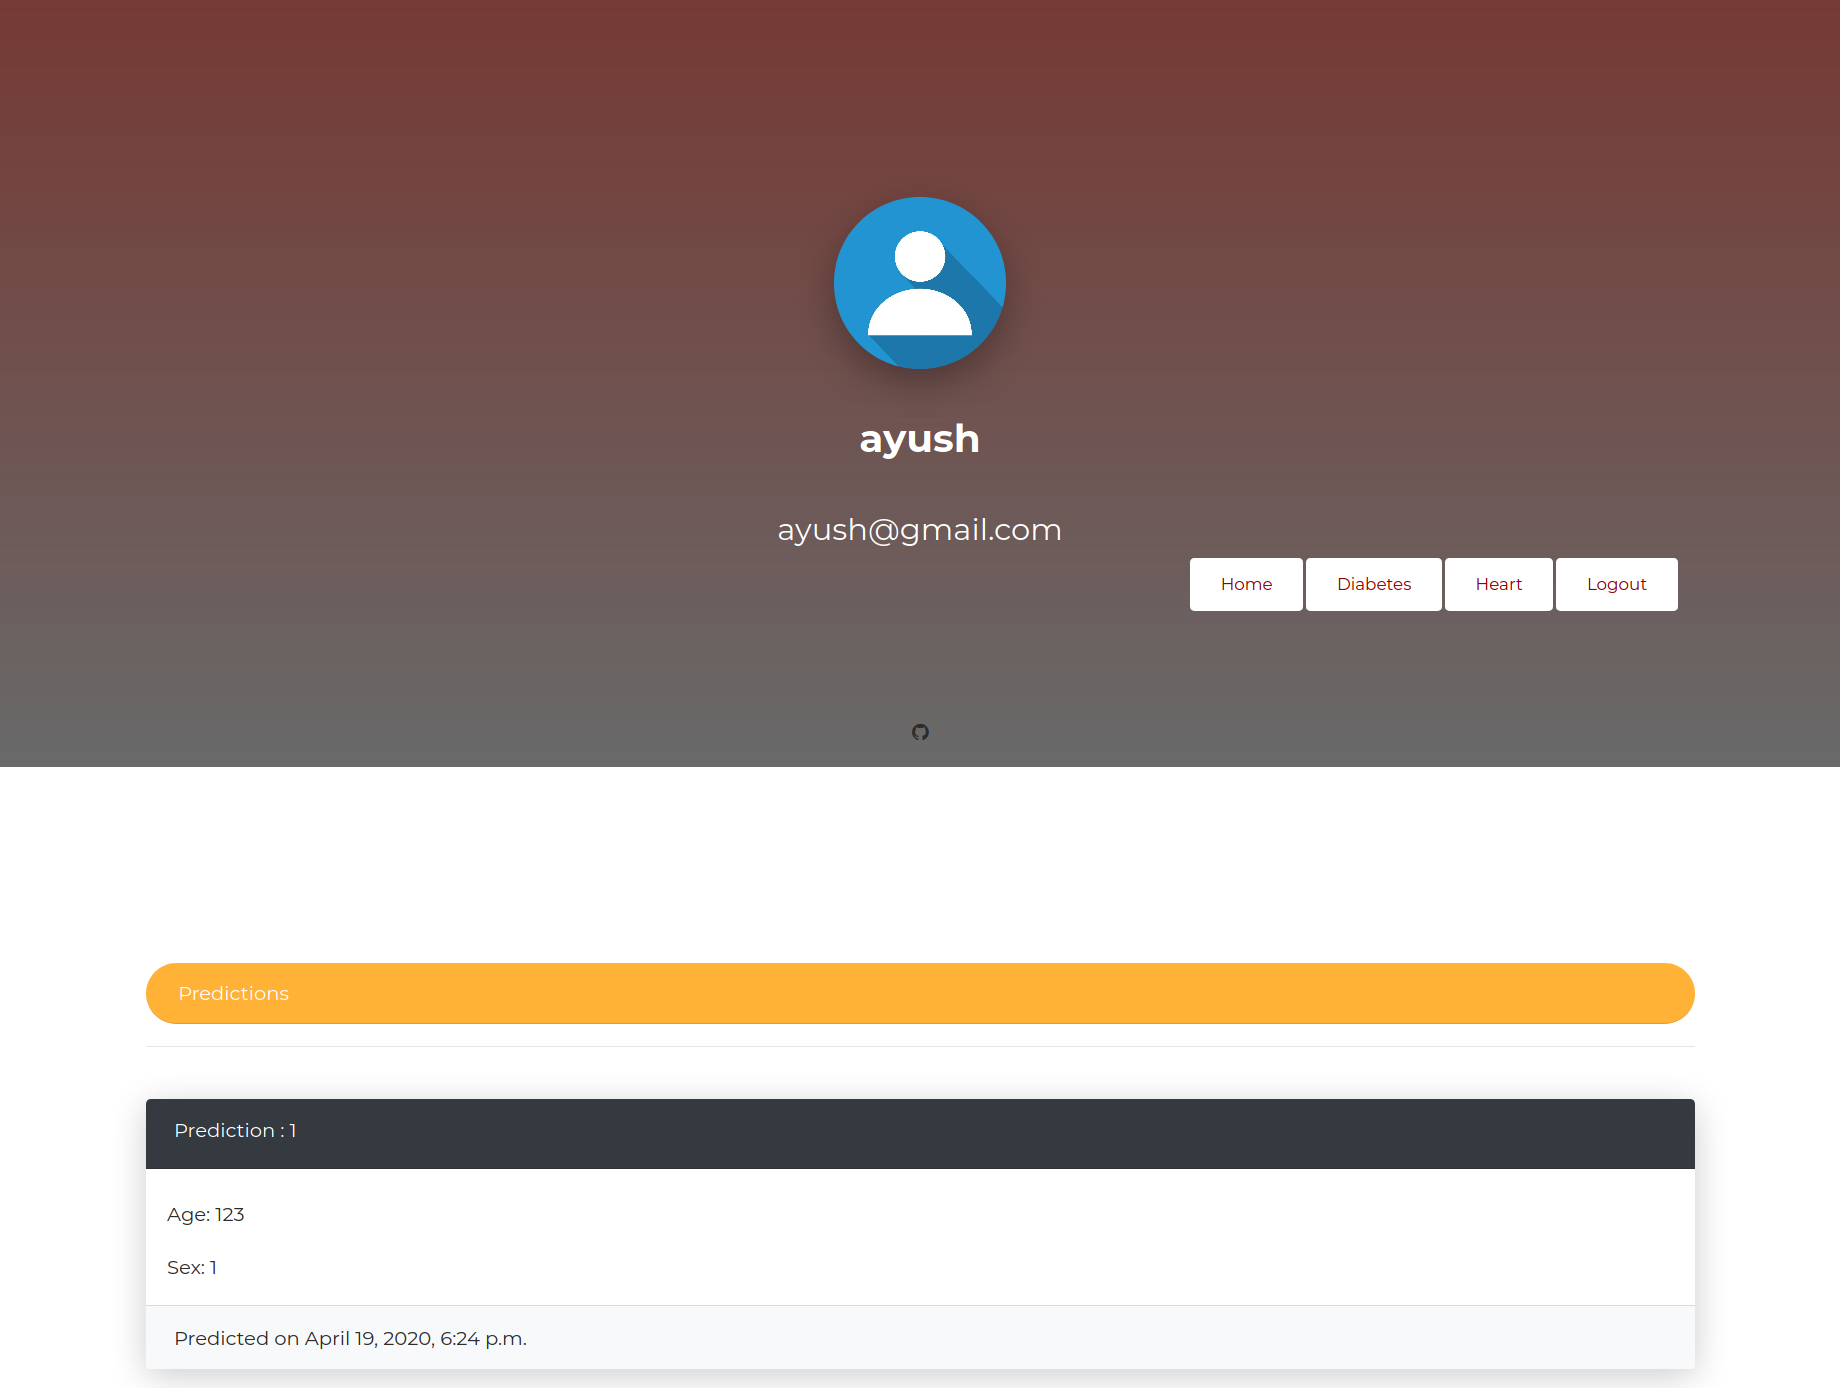
\includegraphics[width=17cm]{Screenshots/profile.PNG}
    				\caption{Profile of a patient showing the past results}
    				\end{center}
    			\end{figure}
    
    \pagebreak
    \section{Data Structures and Algorithms}
    	This section manages data structure and algorithms we have utilized in our project.
    	
    \subsection{Naive Bayes Classifier}
    	Naive Bayes classifiers are a gathering of straightforward probabilistic classifiers based by using Bayes theorem with strong (naive) freedom suppositions between the features. Naive Bayes classifiers are incredibly flexible by requiring different parameters direct for the number of features or pointers as a variable in a learning issue. It is the least perplexing and the snappiest probabilistic classifier, especially for the planning stage.\\ 
    	
    	Naive Bayes classifier depends on Bayes theorem. This classifier utilizes restrictive autonomy wherein characteristic worth is autonomous of the estimations of different qualities. The Bayes theorem is as per the following: 
    	
    	Let X= {x1, x2, ......, Xn} be a lot of n qualities. In Bayesian learning, X is considered as proof and H be some speculation implies, the data of X has a place with explicit class C. We need to decide P (H|X), the likelihood that the speculation H holds given proof, for example, data test X. As indicated by Bayes theorem the P (H|X) is communicated as: \\
    	\[P(H|X) = \frac{P(X|H) * P(H)}{P(X)}\].
    	
    	\begin{figure}[h]
    		\begin{center}
    			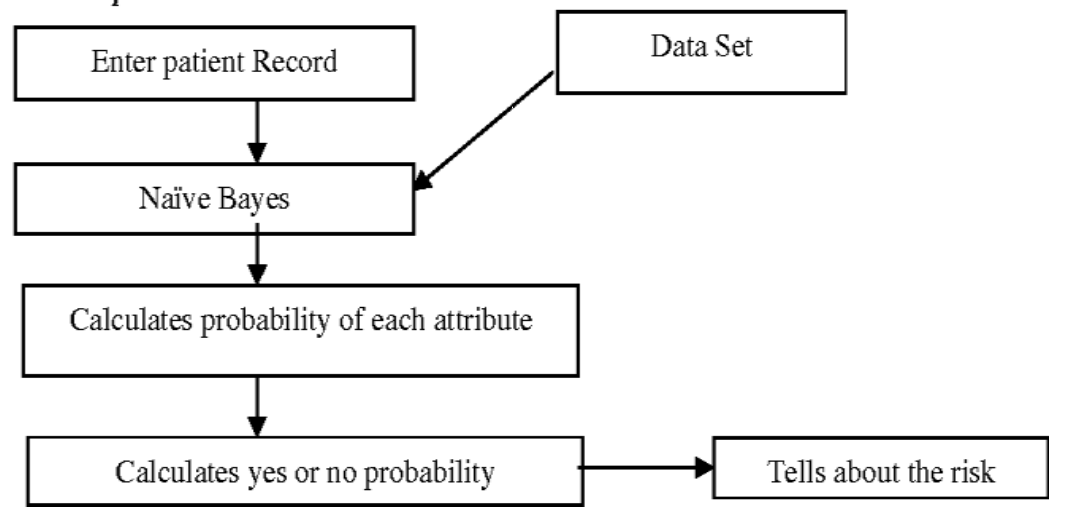
\includegraphics[width = 15cm]{images/naive_bayes.png}\\
    			\caption{Implementation Flow of Naive Bayes Algorithm}
    		\end{center}
    	\end{figure}
    	
       	Utilizing Bayesian classifiers, the framework will find the hidden information related to diseases from authentic records of the patients having heart disease. Bayesian classifiers anticipate the class participation probabilities, such that the likelihood of a given example has a place with a specific class factually. A Bayesian classifier depends on Bayes' theorem. We can utilize Bayes theorem to decide the likelihood that a proposed analysis is right, given the perception. A basic probabilistic, the naive Bayes classifier is utilized for grouping dependent on which depends on Bayes' theorem. As per Naive Bayesian classifier, the event or an event of a specific element of a class is considered as independent in the occurrence or nonoccurrence of some other element. At the point when the element of the sources of info is the high and progressively productive outcome is normal, the boss Naive Bayes Classifier method is appropriate. The Naive Bayes model distinguishes the physical attributes and highlights of patients experiencing heart disease. For each info, it gives the chance of a property of the worthy state. Naive Bayes is a measurable classifier which expects no reliance between properties. This classifier calculation utilizes conditional independence, implies it accept that a quality estimation of a given class is free of the estimations of different qualities. The advantage of using Naive Bayes is that one can work with the Naive Bayes model without utilizing any Bayesian strategies. (Brownlee, 2016). \\ 
       	
       	P (Disease|symptom1, symptom2, ..., symptomn) P(Disease)P(symptom1, ..., symptomn|Disease) = P(symptom1, symptom2, ...symptomnN).\\
    	
    	
    
    
    	\subsection{Decision Tree}
    	Decision tree learning uses a decision tree as a prescient model which maps discernments about a thing to decisions about the thing's objective. It is one of the prescient demonstrating approaches used in estimations, data mining and Artificial Intelligence. Tree models where the target variable can take a limited arrangement of values are called characterization trees. In these tree structures, leaves address class stamps and branches address conjunctions of features that lead to those class names. Decision trees where the target variable can take ceaseless values (customarily real numbers) are called regression trees. In decision tree analysis, a decision tree can be used to apparently and explicitly address decisions and decision making. In data mining, a decision tree portrays data yet not decisions; rather the resulting characterization tree can be a commitment for decision making.\\ 
    	
    	The order tree makes a tree with branches, nodes, and leaves that let us take an obscure data point and plunge the tree, applying the attributes of the data point to the tree until a leaf is reached and the obscure yield of the data point can be resolved. To make a not too bad grouping tree model, we must have a current educational file with known yield from which we can manufacture our model. We also parcel our enlightening assortment into two sections: a preparation set, which is used to construct the model, and a test set, which is used to watch that the model is exact and not overfitted. \\ 
    	
    	This classifier makes a decision tree dependent on which it doles out the class values to every datum point. Here, we can fluctuate the most extreme number of highlights to be thought of while making the model.\\
    	
    		\begin{figure}
    		\begin{center}
    			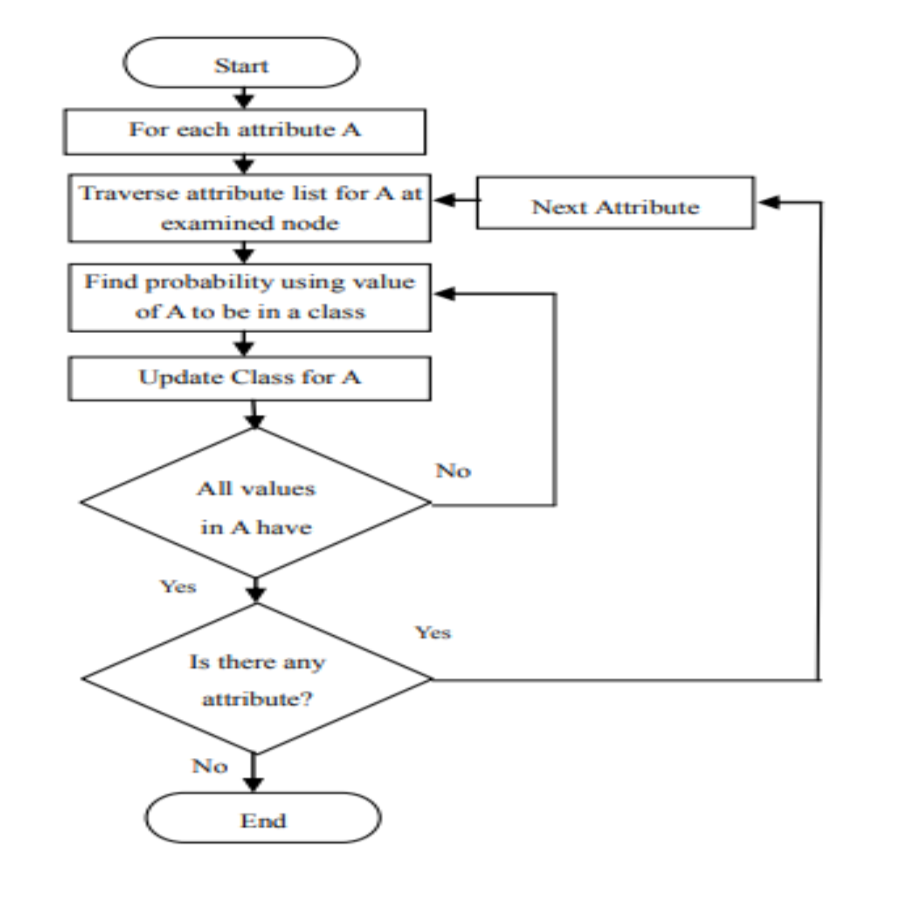
\includegraphics[height=17cm]{images/decision_tree.png}
    			\caption{Flowchart for Decision Tree}
    		\end{center}
    	\end{figure}
    
    	
    	\subsection{Support vector machine(SVM)}
    	SVM was developed by Vladimir Vapnik at AT\&T Bell Labs. It is based on the concept of decision planes that define decision boundaries. A decision plane is a hyperplane that separates the objects having different class memberships. SVM classifiers separate the observations into two or more classes in such a way that maximum separation is achieved. A hypothetical hyperplane is the separator in SVM classification problems.  In other words, SVM constructs a hyperplane that separates the two sets so as to minimize the number of misclassified points. Generally, there are two types of SVM models: linear and nonlinear. Linear SVM works better on linearly separable datasets but nonlinear SVM model works well even on hardly separable datasets. Since we are dealing with hardly separable data in our experiments we use nonlinear SVM. The dual formulation of the nonlinear SVM function can be formulated as
    	\[ MaxW(\alpha) = \sum_{i=1}^{m}\alpha_i - 0.5\sum_{i, j=1}^{m}\alpha_i \alpha_j y_i y_j K(x_i . x_j) \]\\
    	subject to:
    	\[\sum_{i=1}^{m}\alpha_i y_i = 0 ,\]\\
    	\[ 0 \leq \alpha_i \leq C \]\\
    	\begin{figure}
    		\begin{center}
    			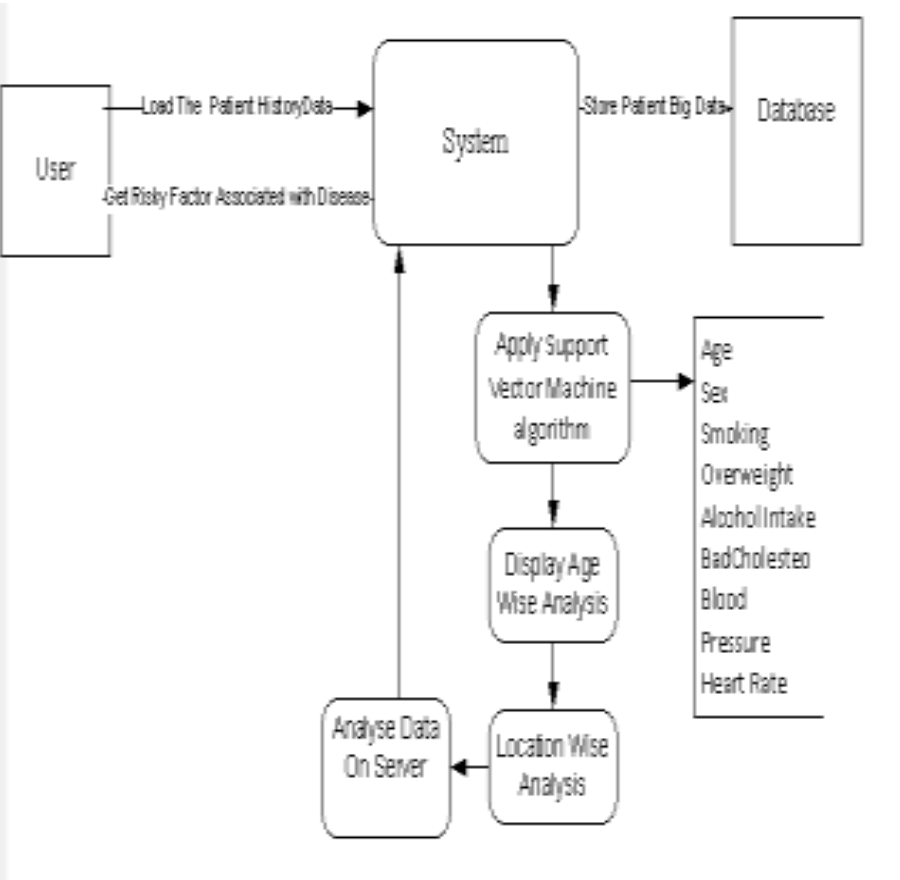
\includegraphics[width=14cm]{images/svm.png}
    			\caption{Flowchart For SVM}
    		\end{center}
    	\end{figure}
    	Input vectors $x_i \in R^m$ , i= 1, 2, 3, …, m, which are called features or attributes are extracted from the database. Associated with every particular input we have a corresponding label ($ y_i = \pm 1$) which is called the target value or output in the database. The variable $\alpha_i$ is the Lagrange multiplier in the dual formulation and C is a user-specified parameter representing the penalty for misclassification K(xi ,xj) is the kernel function and maps the original data points to another space.  One of the popular choices for the kernel is Gaussian kernel which is also known as Radial Basis Function (RBF) in the literature. The formulation for this kernel is
    	\[ K(x_i, x_j) = e^{-\frac{\parallel{x_i - x_j}\parallel^2}{2\sigma}} \]
    	where parameter $\sigma$ is known as the kernel width. 
    	
    	
    	
    	\subsection{Logistic Regression}
    	Logistic Regression is a statistical analysis procedure that is utilized for foreseeing the data esteem dependent on the earlier perception of the data set. The logistic regression model predicts the needy data variable by examining the connection between at least one existing free factors. Logistic Regression is one of the significant instruments for forecast, which can likewise be utilized for characterizing and foreseeing the data dependent on the historical data. The actualized model is a twofold Logistic model that has subordinate factors with just two potential results i.e., one is a positive worth and another is the negative worth which is having 0 or 1 as a class mark.\\ 
    	
    	It for the most part comprises of two significant stages: regularized cost work and regularized angle plummet. Cost Function is utilized for ascertaining the greatest probability estimation. Angle plummet is an iterative procedure for getting coefficients from preparing \\
    	
    	data. The procedure is rehashed until we get the ideal parameters of train data. The model is prepared with the ideal coefficient.Whenever a test data has been passed to the model dependent on the parameters can recognize whether the individual is having coronary illness or not, it tests the data utilizing the sigmoid capacity. The cost work is the technique that is utilized for decreasing the mistakes of the anticipated name and the genuine mark. Slope plunge work is the technique that is utilized for computing the coefficient until we get a base estimation of the class mark.\\
    	
    		
    	\begin{figure}
    		\begin{center}
    			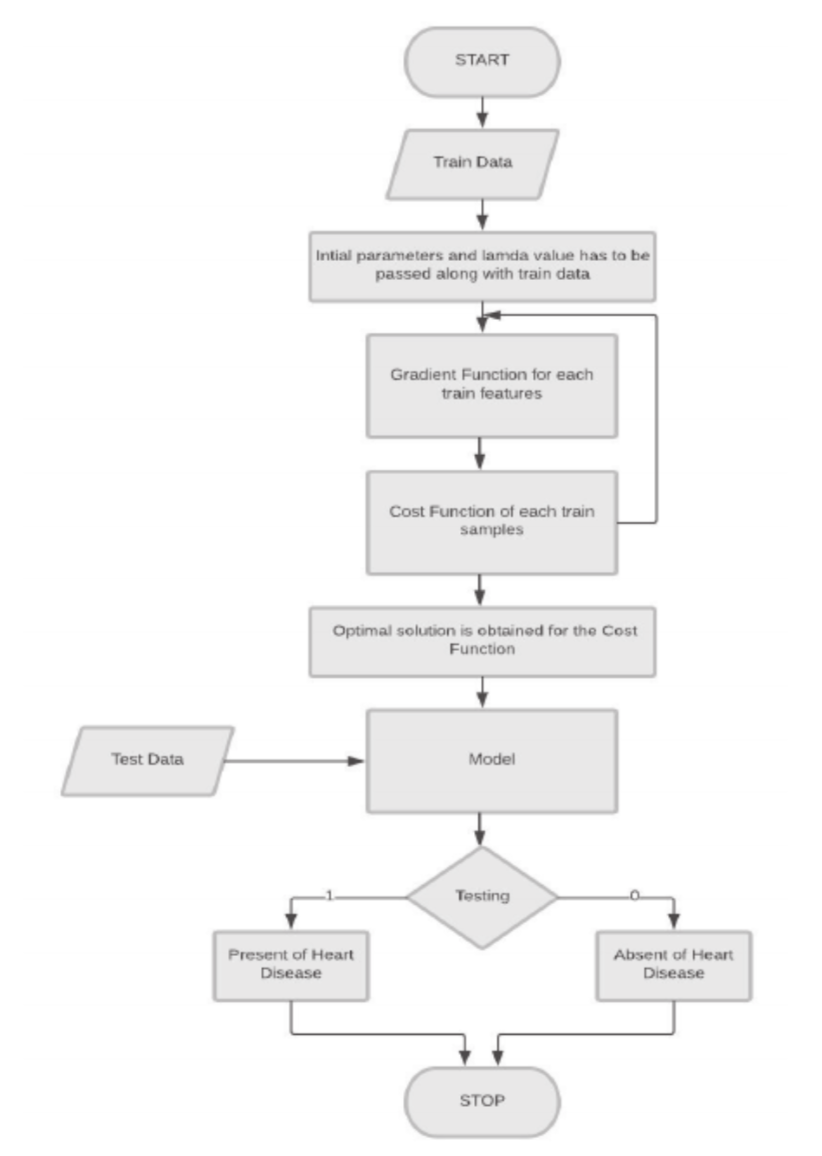
\includegraphics[width=14cm]{images/logistic_regression.png}
    			\caption{FlowChart For Logistic Regression}
    		\end{center}
    	\end{figure}
    	
    	\subsubsection{Cost Function}
    		A minimisation work is used that is the cost work. It uses the Log Loss, for instance, the logarithmic misfortune which evaluates the presence of the model where the figure input regard is the probability between the zero and one. The Log loss is the vulnerability of the forecast which relies upon the sum it changes from the genuine name. Cost work which urges the student to address or change the direction to limit the mistakes. The cost capacity can be surveyed by iteratively running the model to take a gander at the anticipated worth and the known or real worth. The regularized cost work is a method that is used for enduring the risk of overfitting. Lamda is the parameter which controls the regularization term.\\
    		The cost function is calculated by the following:
    		\[ J(\theta) = \frac{1}{m}\sum_{i=1}^{m} y^{(i)} \log[h_\theta(x^{(i)}) - (1-y^{(i)}) \log(1-h_\theta(x^{(i)})] + \frac{\lambda}{2m}\sum_{i=1}^{n}{\theta_j}^2 \] \\
    		m = The number of instances \\
    		n = The number of attributes \\
    		y = The Class label \\
    		x = Features of the training data\\
    		$\theta$ = coefficients \\ 
    		$\lambda$ = learning rate
    	
    	
    	\subsubsection{Gradient Descent}
    		Gradient descent is an advanced strategy which is utilized to discover the parameters or the coefficient of the cost function. Gradient the descent is a rehashed procedure so as to get the coefficients to limit the cost function. The Gradient descent is determined for both the classes to get the pair of a coefficient for both classes marks. The objective here is to proceed with the strategy to attempt the unique esteem for the coefficient, assessing their cost and choosing the new coefficient that is having the somewhat lower cost. Thinking about this coefficient and putting away them in the model. Gradient descent is calculated as follows:
    		\[ \theta_{ji} = \theta_j - \frac{1}{m}\sum_{i=1}^{m}(h_\theta(x^i)-(y^i)) {x_j}^i + \frac{\lambda}{m} \theta_j \]\\
    		m = The number of instances \\
    		x = Features of the training data \\
    		y = The class label \\
    		$\theta$ = coefficients \\
    		$\lambda$ = Learning rate 
    		
    		
    
    	\subsubsection{Sigmoid Function}
    		The sigmoid function is the logistic function between. This takes genuine information vales and yield values between the 0 and 1 for logistic function [12]. This is deciphered as taking log chances and having the yield probability. For the most part, the sigmoid function is utilized to delineate to the probability it is characterized as:
    		\[ h_\theta(x) = \frac{1}{1 + e^{-\theta^{T.x}}} \]\\
    		x = test data features \\
    		$\theta$ = coefficients \\
    		At whatever point a test data is passed it figures the worth dependent on the parameters put away in the model. It computes the probability of each class label. We return the most extreme probability estimation of the class label $x_i$.\\ 
    		
    		The test data contains the thirteen ascribes that we have to pass and compute for both the classes it will restore the two values we take the most extreme estimation of two values we will restore the class with a label which is having the greatest probability.
    	
    	
    	
    		
    		\subsection{K-Nearest Neighbour}  
    		K-Nearest Neighbor (KNN) is a straightforward, lazy and nonparametric classifier. KNN is favoured when all the highlights are consistent. KNN is additionally called case-based thinking and has been utilized in numerous applications like example acknowledgement, statistical estimation. Classification is acquired by distinguishing the nearest neighbour to decide the class of an obscure example. KNN is favoured over other classification algorithms because of its high combination speed and simplicity.\\ 
    		
    		KNN classification has two phases:
    		\begin{enumerate}
    			\item Find the k number of instances in the dataset that is closest to instance S
    			\item These k number of instances then vote to determine the class of instance S
    		\end{enumerate}
    		The Accuracy of KNN relies upon separation metric and K esteem. Different methods of estimating the separation between the two cases are cosine, Euclidean separation. To assess the new obscure example, KNN processes its K nearest neighbours and dole out a class by greater part voting.\\ 
    		
    		With the KNN algorithm, we have the opportunity to change the parameter's weight. It implies that we may accept that a few parameters are more significant or having more effect than others. Among 8 parameters we use, we can classify them our data into 2 classifications, one is "non-clinical" parameters (Age and Sex) and the other is "clinical" parameters (CP, Trestbps, Trestbpd and so forth). We may feel that clinical parameters are a higher priority than non-clinical, which we will see in test results. Alongside weighting, we should discover the estimation of "k" so it gives the best classification result. Since it is a 2-decision classification ("yes") and ("No") k will be an odd number.
    		
    		\begin{figure}
    			\begin{center}
    				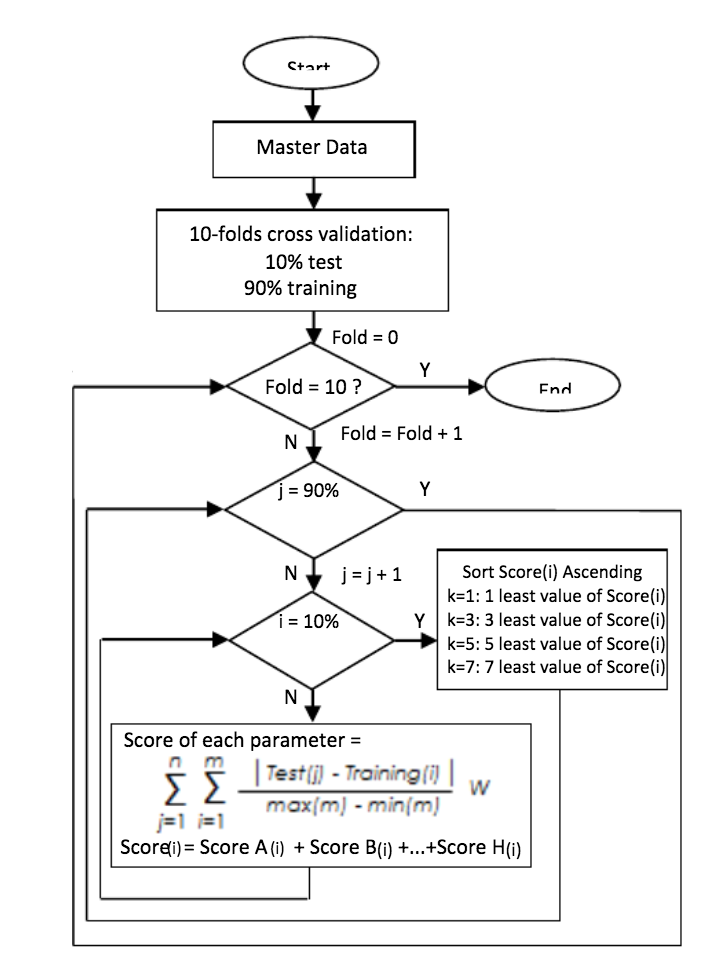
\includegraphics[width=15cm]{images/knn.png}
    				\caption{FlowChart for KNN}
    			\end{center}
    		\end{figure}
    
  		\subsection{Neural Network}
  		\subsubsection{Multilayer Perceptron Neural Network (MLPNN)}
  		One of the most important models in Artificial Neural Network is Multilayer Perceptron
  		(MLP). The  type of architecture  used to  implement  the system  is Multilayer Perceptron Neural Network (MLPNN).
  		\begin{figure}[H]
  			\begin{center}
  				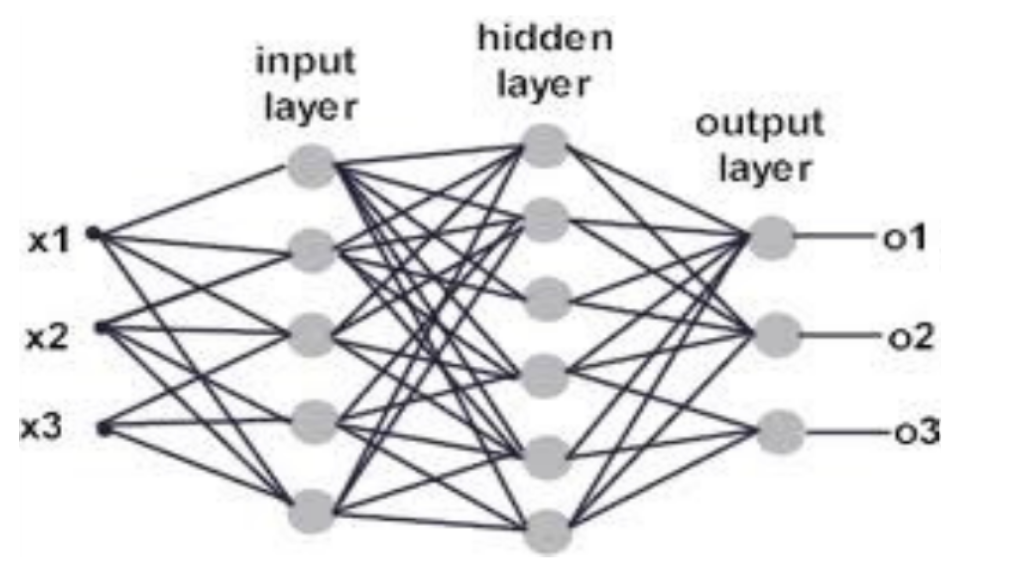
\includegraphics[width=12cm]{images/mlpnn.png}
  				\caption{Neural Network}
  			\end{center}
  		\end{figure}
  		The MLPNN comprises of one input layer, one output layer and at least one hidden layers. Each layer comprises of at least one hubs, spoke to by little circles. The lines between hubs demonstrate stream of data starting with one hub then onto the next hub. The input layer gets signals from outside hubs. The output of input layer is given to hidden layer, through weighted association joins. It performs calculations and transmits the outcome to output layer through weighted connections. The output of hidden layer is sent to output layer, it performs calculations and produce final outcome. The working of multilayer perceptron neural system is summed up in ventures as referenced below:
  		\begin{enumerate}
  			\item Input data is given to the input layer to handling, which creates an anticipated output. 
  			
  			\item The anticipated output is deducted from the real output and blunder esteem is determined. 
  			
  			\item The system at that point utilizes a Backpropagation algorithm which changes the loads. 
  			
  			\item For loads modifying it begins from loads between output layer nodes, what's more, last hidden layer hubs and works in reverse through the system. 
  			
  			\item When back engendering is done, the sending procedure begins once more. 
  			
  			\item The procedure is rehashed until the blunder among the anticipated and real output is limited.
  		\end{enumerate}
  	\pagebreak
  	
  	\subsubsection{Backpropagation network}
  	The most broadly utilized preparing algorithm for multilayer and feed-forward system is Backpropagation. The name given is backpropagation since it computes the distinction among real and anticipated values is proliferated from output hubs in reverse to hubs in the past layer. This is done to improve loads during handling. The working of the Backpropagation algorithm is summed up in ventures as follows:
  	\begin{enumerate}
  		\item Provide preparing data to the network. 
  		\item Compare the genuine and wanted output. 
  		\item Calculate the mistake in every neuron. 
  		\item Calculate what output ought to be for every neuron and how much lower or higher output must be balanced for wanted output. 
  		\item Then alter the loads
  	\end{enumerate}
  
  \begin{figure}
  	\begin{center}
  			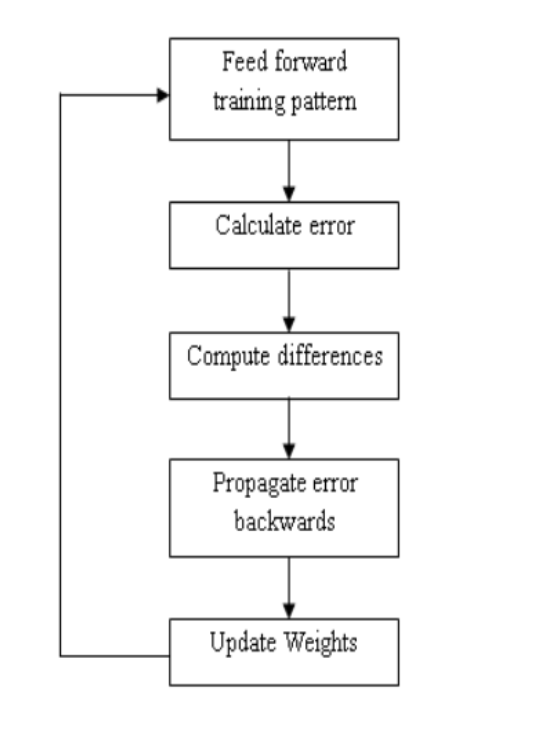
\includegraphics[width=8cm]{images/backpropogation.png}
  			\caption{BackPropagation}
  	\end{center}
  \end{figure}

\begin{figure}[H]
	\begin{center}
		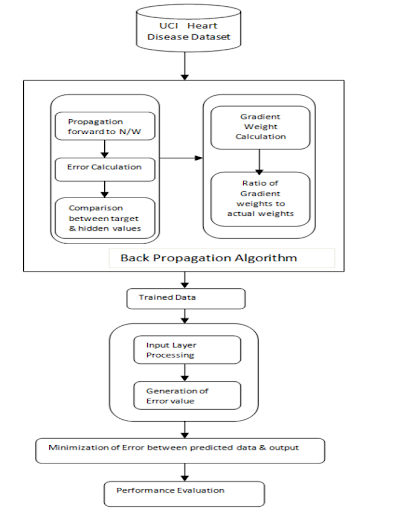
\includegraphics[width=10cm, height=20cm]{images/neural_network.png}
		\caption{Flowchart for Neural Network}	
	\end{center}
\end{figure}

	\section{UML diagrams with discussions} 
	UML is notable for its diagrammatic documentation(Refer Fig 3.10). All in all understand that UML is for imagining, demonstrating, building and recording the portions of programming and non-programming structures. In this way, recognition is the most basic part which ought to be grasped and remembered. UML documentation is the most basic components in illustrating. Viable and reasonable use of documentations is basic for making aggregate and huge model. The model is trivial, with the exception of if its inspiration is depicted really. Subsequently, taking in documentations should be underlined from the most punctual beginning stage. Various documentation is available to things and associations. UML charts are made using the documentations of things and associations. Extensibility is another fundamental part which makes UML even more prevailing and versatile. The model's UML additionally is very instinctive and plain as day, this UML have clear and particular classes which makes it effectively justifiable
	\begin{figure}[h]
		\begin{center}
			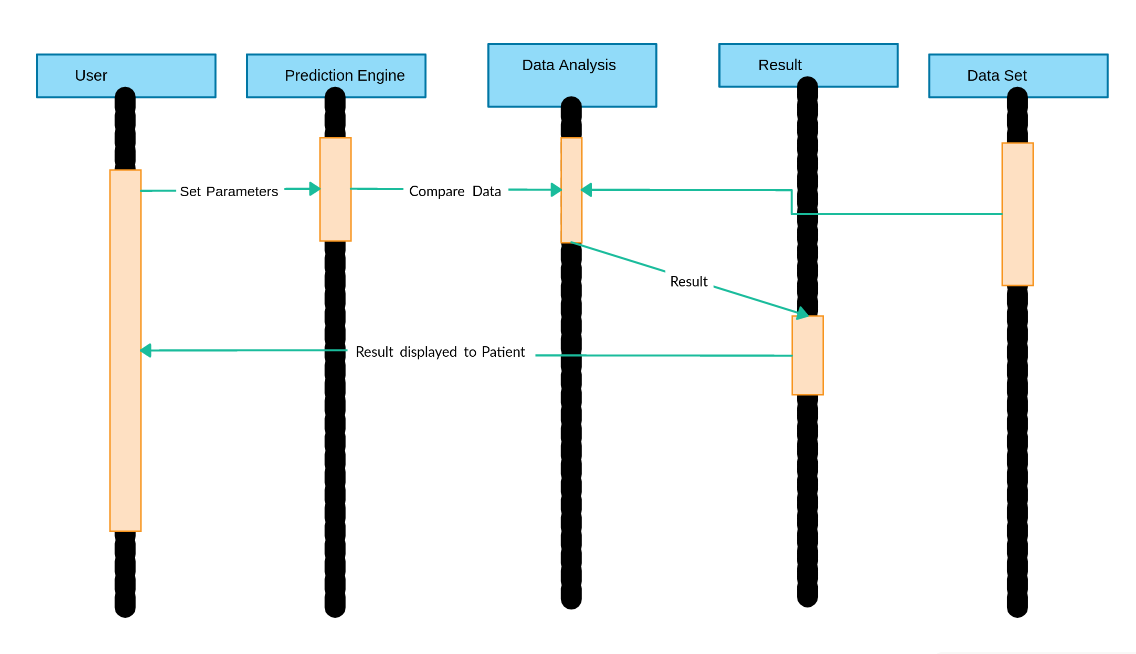
\includegraphics[width=15cm]{images/uml_diagram.png}
			\caption{UML Sequence Diagram}
		\end{center}
	\end{figure}
	
	
	
	






  	
  	\section{Data Source and Formats}
  	\subsection{Heart Disease DataSet}
  	The dataset used in this project is the Cleveland Heart Disease dataset taken from the UCI repository.
  	\begin{center}
  		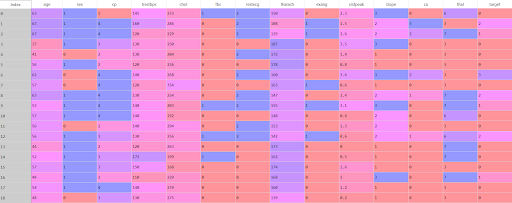
\includegraphics[width=15cm]{images/hdDataset.png}
  	\end{center}
  
  The dataset consists of 303 data points. There are 14 features in the dataset, which are described below.
  \begin{enumerate}
  	\item\textbf{Age:} It consists of the age of the individual.
  	
  	\item \textbf{Sex:} Shows the gender of the individual in the following format:
  		\begin{itemize}
  			\item 1 = Male
  			\item 0 = Female
  		\end{itemize}
  	
  	\item \textbf{Chest-pain type:} displays the type of chest-pain experienced by the individual using the following format :
  		\begin{itemize}
  			\item 1 = typical angina\tiny\textcolor{white}{s}\normalsize
  			\item 2 = atypical angina\tiny\textcolor{white}{s}\normalsize
  			\item 3 = non — anginal pain
  			\item 4 = asymptotic
  		\end{itemize}
  
  	\item \textbf{Resting Blood Pressure}: displays the blood pressure value of an individual in mmHg (unit)
  	
  	\item \textbf{Serum} Cholestrol: displays the serum cholesterol in mg/dl (unit)
  	
  	\item \textbf{Fasting Blood Sugar}: compares the fasting blood sugar value of an individual with 120mg/dl.
  		\begin{itemize}
  			\item If fasting blood sugar > 120mg/dl then, : 1 (true)
  			\item else                                    : 0 (false)
  		\end{itemize}
  	
  	\item \textbf{Resting ECG:} displays resting electrocardiographic results
  	\begin{itemize}
  		\item 0 = normal
  		\item 1 = having ST-T wave abnormality
  		\item 2 = left ventricular hyperthrophy
  	\end{itemize}
  	
  	\item \textbf{Max heart rate achieved:} displays the max heart rate achieved by an individual.
  	\item \textbf{Exercise induced angina\tiny\textcolor{white}{s}\normalsize} :
	  	\begin{itemize}
  			\item 1 = yes
  			\item 0 = no
  		\end{itemize}
  	
  	\item \textbf{ST depression induced by exercise relative to rest:} displays the value which is an integer or float.
  	
  	\item \textbf{Peak exercise ST segment:}
  		\begin{itemize}
	  		\item 1 = upsloping
  			\item 2 = flat
  			\item 3 = downsloping
 	 	\end{itemize}
  	
  	\item \textbf{Number of major vessels (0–3) colored by flourosopy :} displays the value as integer or float.
  	
  	\item \textbf{Thal :} displays the thalassemia :
  		\begin{itemize}
  			\item 3 = normal
  			\item 6 = fixed defect
  			\item 7 = reversible defect
  		\end{itemize}
  	
  	\item \textbf{Diagnosis of heart disease :} Displays whether the individual is suffering from heart disease or not :
  	\begin{itemize}
  		\item 0 = absent
  		\item 1, 2, 3, 4 = present.
  	\end{itemize}
  	
  \end{enumerate}

	\textbf{Why these parameters:}
	In the actual dataset, we had 76 features but for our study, we chose only the above 14 because :
	
	\begin{enumerate}
		\item \textbf{Age:} Age is the most significant hazard factor in creating cardiovascular or heart ailments, with roughly a significantly increasing of hazard with every time of life. Coronary greasy streaks can start to shape in immaturity. It is assessed that 82 per cent of individuals who pass on of coronary illness are 65 and more established. At the same time, the danger of stroke pairs each decade after age 55.
		
		\item \textbf{Sex:} Men are at more serious danger of coronary illness than pre-menopausal ladies. Once past menopause, it has been contended that a lady's hazard is like a man's albeit later data from the WHO and UN questions this. On the off chance that a female has diabetes, she is bound to create coronary illness than a male with diabetes. 
		Angina (Chest Pain): Angina is chest torment or uneasiness caused when your heart muscle doesn't get enough oxygen-rich blood. It might feel like a weight or pressing in your chest. The distress likewise can happen in your shoulders, arms, neck, jaw, or back. Angina torment may even feel like heartburn.
	
		\item \textbf{Resting Blood Pressure:} After some time, high blood pressure can damage supply routes that feed your heart. Hypertension that happens with different conditions, for example, stoutness, elevated cholesterol or diabetes, increases your risk significantly more.
		
		\item \textbf{Serum Cholesterol:} An elevated level of low-thickness lipoprotein (LDL) cholesterol (the "bad" cholesterol) is well on the way to limit conduits. A significant level of triglycerides, a sort of blood fat identified with your eating routine, likewise ups your danger of coronary failure. In any case, a significant level of high-thickness lipoprotein (HDL) cholesterol (the "great" cholesterol) brings down your danger of cardiovascular failure.
		
		\item \textbf{Fasting Blood Sugar:}Not delivering a sufficient hormone emitted by your pancreas (insulin) or not reacting to insulin appropriately causes your body's glucose levels to rise, expanding your danger of cardiovascular failure.
		
		\item \textbf{Resting ECG:} For individuals at generally safe of cardiovascular illness, the USPSTF finishes up with moderate conviction that the potential damages of screening with resting or exercise ECG approach or surpass the potential advantages. For individuals at middle of the road to high hazard, current proof is deficient to evaluate the parity of advantages and damages of screening.
		
		\item \textbf{Max heart rate achieved:} The expansion in cardiovascular hazard, related to the quickening of the pulse, was similar to the increment in chance saw with hypertension. It has been demonstrated that an expansion in pulse by 10 beats for each moment was related with an increment in the danger of cardiovascular passing by in any event 20\%, and this increment in the hazard is like the one saw with an increment in systolic blood pressure by 10 mm Hg.
		
		\item \textbf{Exercise induced angina:} The pain or uneasiness related to angina, for the most part, feels tight, grasping or pressing, and can fluctuate from gentle to extreme. Angina is normally felt in the focal point of your chest however may spread to either or both of your shoulders, or your back, neck, jaw or arm. It can even be felt in your grasp. o Types of Angina a. Stable Angina/Angina Pectoris b. Flimsy Angina c. Variation (Prinzmetal) Angina d. Microvascular Angina.
		
		\item \textbf{Peak exercise ST segment:} A treadmill ECG stress test is viewed as anomalous when there is an even or down-slanting ST-section melancholy $\geq$ 1 mm at 60–80 ms after the J point. Exercise ECGs with up-slanting ST-section miseries are commonly revealed as a 'dubious' test. All in all, the event of flat or down-inclining ST-portion sadness at a lower outstanding task at hand (determined in METs) or pulse shows a more awful guess and a higher probability of multi-vessel malady. The length of ST-portion wretchedness is likewise significant, as drawn-out recuperation after pinnacle pressure is steady with a positive treadmill ECG stress test. Another finding that is profoundly demonstrative of huge CAD is the event of ST-fragment rise > 1 mm (regularly proposing transmural ischemia); these patients often allude desperately for coronary angiography.
	\end{enumerate}

	\subsection{Diabetes DataSet}
	The dataset used in this project is the dataset taken from Kaggle which consist of 768 individual data with 8 column variables.\\
	Description of variables in the dataset:
	\begin{enumerate}
		\item \textbf{Pregnancies:} The number of times the given individual has been pregnant.
		\item \textbf{Glucose:} Plasma glucose concentration over 2 hours in an oral glucose tolerance test.
		\item \textbf{BloodPressure:} Diastolic blood pressure (mm Hg).
		\item \textbf{SkinThickness:} Triceps skin fold thickness (mm).
		\item \textbf{Insulin:} 2-Hour serum insulin (mu U/ml).
		\item \textbf{BMI:} Body mass index $(weight in kg)/(height in m)^2$
		\item \textbf{DiabetesPedigreeFunction:} Diabetes pedigree function(a function which scores likelihood of diabetes based on family history).
		\item \textbf{Age:} Age (years).
		\item \textbf{Outcome:} Class variable.
		\begin{itemize}
			\item 0 = absent
			\item 1 = present
		\end{itemize}
		
	\end{enumerate}
	
	\chapter{Implementation}
	\section{Tools and Technologies}
	\subsection{Django}
	Django styles itself as "an elevated level Python WebApplication system\tiny\textcolor{white}{s}\normalsize that supports fast turn of events and perfect, down to business plan. Worked by experienced creators, it manages an incredible piece of the issue of web improvement, so you can focus on forming your application\tiny\textcolor{white}{s}\normalsize without\tiny\textcolor{white}{s}\normalsize hoping to sit around idly." And they truly would not joke about this! This enormous web system accompanies such a significant number of batteries incorporated that as a rule during advancement it very well may be a riddle concerning how everything figures out how to cooperate. Notwithstanding the system itself being enormous, the Django people group is totally gigantic. Actually, it's so enormous and dynamic that there's an entire site dedicated to the outsider bundles individuals have intended to plug into Django to do an entire host of things. This incorporates everything from confirmation and approval, to all out Django-controlled substance the executives frameworks, to web based business additional items, to combinations with Stripe. Discussion about not re-developing the wheel; odds are on the off chance that you need something finished with Django, somebody has just done it and you can simply maneuver it into your venture.
	\subsection{Python}
	Python is a deciphered, huge stage, comprehensively valuable programming language. Made by Guido van Rossum and first released in 1991, Python's arrangement hypothesis highlights code coherence with its unmistakable usage of colossal whitespace. Its language manufactures and thing arranged procedure expect to help programming engineers with forming clear, genuine code for nearly nothing and huge extension adventures.
	
	Python is progressively composed\tiny\textcolor{white}{s}\normalsize and trash\tiny\textcolor{white}{s}\normalsize gathered. It\tiny\textcolor{white}{s}\normalsize bolsters various programming standards, including organized (especially, procedural), object-arranged, and hands-on programming. Python is regularly portrayed as\tiny\textcolor{white}{s}\normalsize a "batteries included" language\tiny\textcolor{white}{s}\normalsize because\tiny\textcolor{white}{s}\normalsize of its extensive standardised library. 
	
	Python was considered in the late 1980s as a substitution to the ABC language. Python 2.0, released in 2000, introduced features like overview understandings and a refuse combination system fit for social occasion reference cycles. Python 3.0, released in 2008, was a huge revision of\tiny\textcolor{white}{s}\normalsize the language\tiny\textcolor{white}{s}\normalsize that\tiny\textcolor{white}{s}\normalsize isn't absolutely\tiny\textcolor{white}{s}\normalsize in invert\tiny\textcolor{white}{s}\normalsize great.
	
	\subsection{SqlLite}
	SQLite is a little database application that is utilized in a great many programming and gadgets. SQLite was concocted by D.Richard Hipp\tiny\textcolor{white}{s}\normalsize in August\tiny\textcolor{white}{s}\normalsize 2000. SQLite is an elite, lightweight social database. In the event that you are happy to get familiar with the internals\tiny\textcolor{white}{s}\normalsize of\tiny\textcolor{white}{f}\normalsize a database\tiny\textcolor{white}{s}\normalsize at a coding\tiny\textcolor{white}{s}\normalsize stages, at that point SQLite is the best open-source database accessible out there with profoundly coherent source code with bunches of documentation. SQLite\tiny\textcolor{white}{s}\normalsize database engineering split\tiny\textcolor{white}{s}\normalsize into\tiny\textcolor{white}{s}\normalsize two unique segments named as center and backend. Center segment contains Interface, Tokenizer, Parser, Code generator, and the virtual machine, which make an\tiny\textcolor{white}{y}\normalsize execution request for\tiny\textcolor{white}{m}\normalsize database exchanges. Backend contains B-tree, Pager and OS interface to get to the document framework. Tokenizer\tiny\textcolor{white}{s}\normalsize , Parser\tiny\textcolor{white}{s}\normalsize and code\tiny\textcolor{white}{s}\normalsize generator\tiny\textcolor{white}{f}\normalsize out and out named as the compiler which creates a lot of opcodes\tiny\textcolor{white}{s}\normalsize that sudden spikes in demand for a virtual machine.
	
	\subsection{IntelliJ IDEA}
	IntelliJ IDEA\tiny\textcolor{white}{s}\normalsize is\tiny\textcolor{white}{s}\normalsize a integrated\tiny\textcolor{white}{s}\normalsize development\tiny\textcolor{white}{s}\normalsize environment (IDE) written\tiny\textcolor{white}{s}\normalsize in Java\tiny\textcolor{white}{s}\normalsize for creating PC programming. It is created by JetBrains (once in the past known as IntelliJ), and is\tiny\textcolor{white}{s}\normalsize accessible\tiny\textcolor{white}{s}\normalsize as an Apache 2 Licensed people\tiny\textcolor{white}{s}\normalsize group\tiny\textcolor{white}{s}\normalsize version, and in an exclusive business release. Both can be used for bussiness advancement. The IDE gives certain highlights like code fruition by\tiny\textcolor{white}{y}\normalsize investigating\tiny\textcolor{white}{s}\normalsize the unique situation, code route which permits bouncing to\tiny\textcolor{white}{s}\normalsize classes or\tiny\textcolor{white}{s}\normalsize statement in the code straightforwardly, code refactoring, code troubleshooting , linting and choices to fix irregularities through proposals. The IDE furnishes mix with construct/bundling devices like snort, grove, gradle\tiny\textcolor{white}{s}\normalsize , and SBT. It bolsters adaptation control frameworks like Git, Mercurial, Perforce, and SVN. Databases like Microsoft SQL Server, Oracle, PostgreSQL, SQLite and MySQL can be gotten to straightforwardly from\tiny\textcolor{white}{s}\normalsize the IDE\tiny\textcolor{white}{s}\normalsize in the Ultimate\tiny\textcolor{white}{s}\normalsize release, through\tiny\textcolor{white}{t}\normalsize an inserted variant of DataGrip. IntelliJ\tiny\textcolor{white}{s}\normalsize underpins modules through\tiny\textcolor{white}{t}\normalsize which one\tiny\textcolor{white}{s}\normalsize can\tiny\textcolor{white}{s}\normalsize add extra usefulness to the IDE. Modules can be downloaded and introduced either from IntelliJ's module store site or through\tiny\textcolor{white}{t}\normalsize the\tiny\textcolor{white}{y}\normalsize IDE's inbuilt\tiny\textcolor{white}{s}\normalsize module look and introduce highlight. Every version has separate module storehouses, with both\tiny\textcolor{white}{s}\normalsize the\tiny\textcolor{white}{y}\normalsize Community\tiny\textcolor{white}{es}\normalsize and Ultimate\tiny\textcolor{white}{f}\normalsize releases totaling more than 3000 modules each starting at 2019..
	
	\subsection{Machine Learning}
	A better than average start at a Machine Learning definition is that it is a middle sub-territory of Artificial Intelligence (AI). ML applications gain for a reality (well data) like individuals without direct programming. Exactly when introduced to new data, these applications learn, create, change, and make without any other person. All things considered, with Machine Learning, PCs discover astute information without being exhorted where to look. Or maybe, they do this by using computations that gain from data in an iterative technique.
	
	While the idea\tiny\textcolor{white}{s}\normalsize of Machine\tiny\textcolor{white}{f}\normalsize Learning\tiny\textcolor{white}{f}\normalsize has been\tiny\textcolor{white}{s}\normalsize around\tiny\textcolor{white}{s}\normalsize for\tiny\textcolor{white}{m}\normalsize quite a while (think about the WWII Enigma Machine), the capacity to robotize the use of complex scientific estimations to Big Data has been picking up energy in the course of the most recent quite a long while. 
	
	At a significant level, Machine\tiny\textcolor{white}{f}\normalsize Learning\tiny\textcolor{white}{g}\normalsize is the capacity to\tiny\textcolor{white}{e}\normalsize adjust\tiny\textcolor{white}{s}\normalsize to new\tiny\textcolor{white}{s}\normalsize information  freely and through emphasess. Fundamentally, applications gain from past\tiny\textcolor{white}{s}\normalsize calculations and exchanges and use "design\tiny\textcolor{white}{s}\normalsize acknowledgment\tiny\textcolor{white}{s}\normalsize " to deliver\tiny\textcolor{white}{s}\normalsize dependable and educated outcomes.
	\subsection{HTML}
	Hypertext\tiny\textcolor{white}{f}\normalsize Markup\tiny\textcolor{white}{f}\normalsize Language\tiny\textcolor{white}{s}\normalsize (HTML) is the standard\tiny\textcolor{white}{s}\normalsize markup language for archives intended to be displayed in an internet\tiny\textcolor{white}{s}\normalsize browser. It very well may be helped\tiny\textcolor{white}{s}\normalsize by advancements, for example, Cascading\tiny\textcolor{white}{s}\normalsize Style Sheets (CSS) and scripting\tiny\textcolor{white}{s}\normalsize languages, for example, JavaScript. 
	
	Web programs get HTML chronicles from a web server or from neighborhood amassing and render the reports into intuitive media site pages. HTML depicts the structure of a site page semantically and at first included signs for the presence of the report.
	
	HTML parts are the structure squares of HTML pages. With HTML creates, pictures and various articles, for instance, natural structures may be introduced into the rendered page. HTML gives an approach to make composed documents by significance assistant semantics for content, for instance, headings, sections, records, associations, refers to and various things. HTML parts are depicted by names, made using point segments. Marks, for instance, <img/> and <input/> direct carry content into the page. Various names, for instance, <p> envelop and give information about record message and may join various names as sub-parts. Projects don't show the HTML marks, yet use them to decipher the substance of the page.
	
	\subsection{Cascading Style Sheets}
	Cascading\tiny\textcolor{white}{s}\normalsize Style Sheets (CSS) is a template language used\tiny\textcolor{white}{s}\normalsize for depicting the presentation of a chronicle written in a markup\tiny\textcolor{white}{s}\normalsize language like HTML. CSS is an establishment development of the World Wide Web, near to HTML and JavaScript. CSS is proposed to engage the parcel of presentation and substance, including configuration, tones, and literary styles. This parcel can improve content receptiveness, give more prominent versatility and control in the assurance of presentation\tiny\textcolor{white}{s}\normalsize characteristics\tiny\textcolor{white}{s}\normalsize , engage different site pages to share masterminding by demonstrating the critical CSS in an alternate .css report, and lessen eccentrics and emphasis in the\tiny\textcolor{white}{s}\normalsize essential substance\tiny\textcolor{white}{s}\normalsize .
	
	\section{Experimental Setup}
	\begin{enumerate}
		\item 10th Generation Intel® Core™ i7\tiny\textcolor{white}{s}\normalsize Processors 8M\tiny\textcolor{white}{B}\normalsize Cache\tiny\textcolor{white}{s}\normalsize , up to 3.90 GHz
		\item Disk space 1TB.
		\item Operating System: Linux 18.04. 
	\end{enumerate}
	
	\textbf{Recommended System Requirements}  
	
	\begin{itemize}
		\item Intel® Core™ i5-8257U Processor 6M\tiny\textcolor{white}{B}\normalsize Cache, up to 3.90 GHz\tiny\textcolor{white}{s}\normalsize , 8 GB of DRAM. 
		\item Operating systems:  Linux 18.04.
	\end{itemize}
	
	\textbf{Minimum System Requirements}
	
	\begin{enumerate}
		\item Processors: Intel Atom®\tiny\textcolor{white}{f}\normalsize processor\tiny\textcolor{white}{f}\normalsize or Intel® Core™ i3 processor.
		\item Disk\tiny\textcolor{white}{s}\normalsize space: 1 GB 
		\item Operating\tiny\textcolor{white}{s}\normalsize systems: Windows* 7 or later\tiny\textcolor{white}{f}\normalsize, macOS, and Linux 
		\item Python*\tiny\textcolor{white}{s}\normalsize versions: 2.7.X, 3.6.X 
		\item Included\tiny\textcolor{white}{s}\normalsize development tools: conda*, conda-env, Jupyter Notebook* (IPython) 
		\item Compatible\tiny\textcolor{white}{s}\normalsize tools: Microsoft\tiny\textcolor{white}{s}\normalsize Visual Studio*, PyCharm*Included\tiny\textcolor{white}{s}\normalsize Python packages - NumPy, SciPy, scikit-learn*, pandas, Matplotlib, Numba*\tiny\textcolor{white}{s}\normalsize, Intel® Threading\tiny\textcolor{white}{s}\normalsize Building Blocks\tiny\textcolor{white}{s}\normalsize , pyDAAL, Jupyter, mpi4py, PIP*\tiny\textcolor{white}{s}\normalsize , and other 
	\end{enumerate}
	\section{Coding Standards followed}
	With regards to the coding styles or coding principles, Developers have wide scope of adaptability, based on a few parameters, be it any plan. A decent structured code as that in the present task considers the following\tiny\textcolor{white}{s}\normalsize :
	\begin{itemize}
		\item prper documentation\tiny\textcolor{white}{s}\normalsize has been done by comments
		\item caode is been refactored and extra spaces has been removed 
		\item proper libary has been imported
		\item proper message hass been added while commiting the code 
		\item proper naming conventions has been followed
		\item meaningful variable names has been used
		\item OOP concept has been used 
		\item Code is written in a genral for proper re-usabilty 
	\end{itemize}
	
	\section{Code Integration details}
	The integration of code has been finished utilizing GIT as the form control. The python code has been well packed in modules which\tiny\textcolor{white}{s}\normalsize has\tiny\textcolor{white}{s}\normalsize provided ease\tiny\textcolor{white}{s}\normalsize of\tiny\textcolor{white}{f}\normalsize integration\tiny\textcolor{white}{s}\normalsize . The HTML forms are provided by means of python class by creating object for each input entity and adding constraints to those classes which makes the HTML page dynamic and easy to adapt new changes. The design of our developed project is such that files names and location are specified through regex. The modules are enclosed in packages which increase the readability and simplicity of code. The machine learning algorithms uses a file to read new data provided by user and to predict the result. This prediction result is passed to the prediction page through a data provider class. The prediction data is stored in database for keeping track of predictions.
	
	\section{Implementation work flow}
	Implementation considers sort of calculation utilized in the task, its proficiency, with the goal that the utilization of the most conceivable proficient algorithms can be utilized, in view of the utilization case, designers and the developers group. This undertaking has been worked over comparative meaning of usage, wherein every part of execution has been dealt with, directly from the structure of the UI to database, calculations to programming interface . A specific structure design has been followed to advance adaptability and legitimate support of the code. The work process begins directly from the plan execution and finishes on code usage. Algorithms has been utilized which figures the chance of sicknesses dependent on the input gave by the patient. Authentication and validation of client information has been considered and all the historical backdrop of searches made are put away in the database with timestamp.
	\subsection{Data cleaning}
	Information cleaning undertakings utilizing Python's Pandas library. In particular, we've center around most likely the greatest information cleaning task, missing attributes values.
	\subsubsection{Sources of Missing Values}
	\begin{itemize}
		\item User\tiny\textcolor{white}{s}\normalsize forgot\tiny\textcolor{white}{s}\normalsize to fill in a field.
		\item Data was lost\tiny\textcolor{white}{s}\normalsize while transferring\tiny\textcolor{white}{s}\normalsize manually\tiny\textcolor{white}{s}\normalsize from a legacy\tiny\textcolor{white}{s}\normalsize database\tiny\textcolor{white}{s}\normalsize.
		\item Error in Programming.
		\item Users decided not to round out a field attached to their convictions about how the outcomes would be utilized or deciphered.
	\end{itemize}
	On the off chance that we investigate the coloums of dataset,we can see that Pandas occupied in the blanked space with "NA". Utilizing the isnull() strategy, we can affirm that both the missing worth and "NA" were perceived as missing qualities. Both boolean reactions are True. Pandas will perceive both void cells and "NA" types as absent values.But there are estimations of certain sorts that Pandas won't recognize.
	\subsubsection{Non-Standard Missing Values}
	On the off chance that there's numerous clients physically entering information, at that point this is a typical issue. Possibly some prefer to utilize "n/a" yet other like to utilize "na". A simple method to recognize these different configurations isto placed them\tiny\textcolor{white}{!}\normalsize in a\tiny\textcolor{white}{s}\normalsize list. At that point when we import the data, Pandas will remember them right\tiny\textcolor{white}{s}\normalsize away\tiny\textcolor{white}{ed}\normalsize . Below is the case of how its done here.
	\begin{figure}
		\begin{center}
			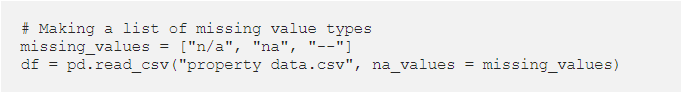
\includegraphics[width=8cm]{images/datacleaning.PNG}
			\caption{making a list of missing values}
		\end{center}
	\end{figure}
	
	\subsection{Handling unstructured and structured Data} Python supports good libraries for handling structured and unstructured data
	\begin{itemize}
		\item \textbf{Python processing CSV data}
		\begin{itemize}
			\item The csv document is a text record in which the qualities in the columns are isolated by a comma. How about we consider the accompanying information present in the record named input.csv.
			\item we can make this record utilizing windows notebook by reordering this information. Spare the document as input.csv
			\item The read csv capacity of the pandas library is utilized perused the contents of a CSV document into the python condition as a pandas DataFrame. The method can peruse the records from the OS by utilizing appropriate way to the file.
			\item The read csv method of the pandas library can likewise be utilized to peruse some particular lines for a given section.
		\end{itemize} 
		\item \textbf{Python processing JSON data}
		\begin{itemize}
			\item Make a JSON record by duplicating the beneath information into a content tool like scratch pad. Spare the document with .json expansion
			\item The read json function\tiny\textcolor{white}{s}\normalsize of\tiny\textcolor{white}{f}\normalsize the\tiny\textcolor{white}{y}\normalsize pandas library\tiny\textcolor{white}{es}\normalsize can be used to read the JSON file into a pandas DataFrame. 
			\item the read json capacity of the pandas library can likewise be utilized to understand a specific columns and specific rows after the JSON file is read to a DataFrame. We use the multi-axes indexing method called .loc $($ $)$ for this purpose.
			\item We can also apply the tojson function along with parameters to read the JSON file content into individual records.
		\end{itemize} 
	\end{itemize}
	
	\section{Execution Results and Discussions}
	The consequences of\tiny\textcolor{white}{f}\normalsize execution\tiny\textcolor{white}{f}\normalsize of\tiny\textcolor{white}{f}\normalsize the code\tiny\textcolor{white}{s}\normalsize are very good. A total flow of\tiny\textcolor{white}{f}\normalsize the\tiny\textcolor{white}{y}\normalsize application\tiny\textcolor{white}{s}\normalsize could been watched, with no deadly mistake and code break. A portion of the occasions are as per the following:
	\begin{itemize}
		\item User are able to signup with email and password
		\item Existing user are able to login with valid email and password of more the length of 6 characters
		\item User\tiny\textcolor{white}{s}\normalsize must able to predict heart disease 
		\item User\tiny\textcolor{white}{s}\normalsize must able to predict diabetes  
		\item User\tiny\textcolor{white}{s}\normalsize shoulc able to move to the contact page of development team by clicking on contact button 
		\item User should be able to logout from its account succesfully 
		
	\end{itemize}
	\section{Non-functional requirements results}
	\begin{enumerate}
		\item \textbf{Performance parameters} This incorporates the reaction time of the framework usage level of both\tiny\textcolor{white}{s}\normalsize static\tiny\textcolor{white}{s}\normalsize and volumetric sort throughput and so forth these\tiny\textcolor{white}{f}\normalsize parameters\tiny\textcolor{white}{f}\normalsize are normalized so a framework needs to tail them
		\item \textbf{Corrective Maintenance} In case of any bugs left in the system, the bugs and issues will be fixed for smooth running of application. The accuracy of the system can be further improved with other algorithm if needed
		\item \textbf{Adaptive maintenance} The features in the applications can be added sauch as history of the disease can be kept in the log. the available list of symptoms can also be added for covering more number of diseases.
		\item \textbf{Security} Amazon web administrations utilizes a few operational security highlights like powerlessness managements, malware anticipation, checking, incident management, server and programming stack security, believed server boot, made sure about help APIs and verified access, information encryption, organize firewall rule upkeep.
		\item \textbf{Interoperability} This requirement demands the system to be built so that it can work in joining with different operating\tiny\textcolor{white}{s}\normalsize systems\tiny\textcolor{white}{s}\normalsize and can be\tiny\textcolor{white}{en}\normalsize changed\tiny\textcolor{white}{f}\normalsize as per\tiny\textcolor{white}{s}\normalsize the user requirements.Since the end product of this project is a web app hosted on AWS cloud, therefore the web app can be accessed by any user on any device through the internet. 
	\end{enumerate}
	
	
	\chapter{Testing}
	
	\section{Test workflow}
	\subsection{Integration Testing}
	Testing for the integration of components of the application. This kind of testing is done after the application is entirely evolved, so as to check the integration with all the limit cases considered. An application is said to pass the integration testing just when all the components are incorporated to one another with an undeniable stream, and the code doesn't break over any module or segment. This testing is done commonly through mechanization as manual testing concerning integration would not test the equivalent on various parameters dependent on ongoing information.
	
	\subsection{Unit Testing}
	This kind of\tiny\textcolor{white}{f}\normalsize testing\tiny\textcolor{white}{s}\normalsize manages testing\tiny\textcolor{white}{s}\normalsize of\tiny\textcolor{white}{f}\normalsize each class, technique or bussiness rationale as a unit. Unit\tiny\textcolor{white}{s}\normalsize testing\tiny\textcolor{white}{s}\normalsize is one\tiny\textcolor{white}{y}\normalsize of\tiny\textcolor{white}{f}\normalsize the incredible strategies for testing which advances free coupling\tiny\textcolor{white}{s}\normalsize as every bit of utilization case\tiny\textcolor{white}{s}\normalsize as a\tiny\textcolor{white}{s}\normalsize business rationale is kept up as a nuclear unit\tiny\textcolor{white}{y}\normalsize. No two techniques have some\tiny\textcolor{white}{s}\normalsize usefulness. Not withstanding that a strategy is planned uniquely to deal with one use\tiny\textcolor{white}{s}\normalsize case\tiny\textcolor{white}{y}\normalsize . The strategies just hold\tiny\textcolor{white}{s}\normalsize bussines rationale decoupled from\tiny\textcolor{white}{y}\normalsize any\tiny\textcolor{white}{y}\normalsize device components, explicitly android for our situation. In the application\tiny\textcolor{white}{s}\normalsize , MVP configuration design has been utilized which\tiny\textcolor{white}{y}\normalsize is the\tiny\textcolor{white}{y}\normalsize most capable plan design with regards to unit testing. This design has been utilized in light of the fact that it makes\tiny\textcolor{white}{y}\normalsize the\tiny\textcolor{white}{y}\normalsize business rationale liberated from the android\tiny\textcolor{white}{y}\normalsize components and makes it simpler to perform\tiny\textcolor{white}{y}\normalsize unit\tiny\textcolor{white}{y}\normalsize testing\tiny\textcolor{white}{y}\normalsize with no coupling. All the system calls have been done in the moderator layer, wherein the view layer is obscure of\tiny\textcolor{white}{f}\normalsize the system calls and\tiny\textcolor{white}{i}\normalsize related information. The moderator is put\tiny\textcolor{white}{s}\normalsize to test as\tiny\textcolor{white}{y}\normalsize and when\tiny\textcolor{white}{y}\normalsize required\tiny\textcolor{white}{y}\normalsize .
	
	\subsection{Validation Testing}
	It begins around the finishing of coordination testing when explicit parts have been worked out, the thing is completely assembled as a group, and interfacing messes up have been uncovered and redressed. At the support or framework level, the capacity between normal programming, battle engineered programming and WebApps vanishes. The path toward investigating programming in the midst of the change framework or toward the aggregate of the advancement strategy to pick in the event that it satisfies picked business necessities. It ensures that the module truly addresses the client's issues. It can in like manner be depicted as to show that the thing fulfills its run of the mill use when sent on reasonable condition. It reacts to the request, Are we making the right thing?
	
	\section{Test case details}
	\subsection{Test case 1:}
	Unit\tiny\textcolor{white}{s}\normalsize to test\tiny\textcolor{white}{d}\normalsize : User\tiny\textcolor{white}{y}\normalsize Authentication\tiny\textcolor{white}{s}\normalsize \\
	Assumptions\tiny\textcolor{white}{s}\normalsize :\\
	\begin{itemize}
		\item Patient is\tiny\textcolor{white}{s}\normalsize a first time\tiny\textcolor{white}{s}\normalsize user
		\item Patient may be an existing\tiny\textcolor{white}{s}\normalsize user
		\item He/She enters the\tiny\textcolor{white}{y}\normalsize correct\tiny\textcolor{white}{s}\normalsize password which\tiny\textcolor{white}{s}\normalsize belongs to him/her
	\end{itemize}
	Test data: minimum six digit passwors\\
	\\
	Steps executed:
	\begin{itemize}
		\item A first time\tiny\textcolor{white}{s}\normalsize user\tiny\textcolor{white}{s}\normalsize enters his/her username, email, password, confirm password
		\item Following the above, he/she clicks on the submit button
		\item Moves to the home page of the web app
	\end{itemize}
	Expected result:
	\begin{itemize}
		\item user should be redirected to the home page of the web app where he/she gets option to predict heart or diabeties disease
	\end{itemize}
	Actual result:when user enters first time and signUp with email and password, he shoud be redirected to the home page\\
	\\
	Result(Pass or Fail): Passed\\
	\\
	Comments: The test passed successfully and everything worked fine
	
	\subsection{Test case 2:}
	Unit to test: verification of home page details\\
	Assumptions:\\
	\begin{itemize}
		\item Patient is a first time user
		\item Patient may be an existing user
		\item He/She enters the correct password which belongs to him/her
	\end{itemize}
	Test data: user should have login with correct username and password\\
	\\
	Steps to be executed:\\
	\begin{itemize}
		\item Home page should have buttons for heart diseases prediction and diabeties prediction
		\item It should also contains all the navigable buttons in the top corners of website
		\item Moves to the corresponding page of the web app when any button is clicked.
	\end{itemize}
	Expected result:  Moves to to the corresponding page of the application when click on any button.\\
	\\
	Actual result: The user was able to navigate throughout the website\\
	\\
	Result(Pass or Fail): Passed\\
	\\
	
	\subsection{Test case 3:}
	Unit to test: database storage of patients\\
	Assumptions:\\
	\begin{itemize}
		\item Admin user name and password.
	\end{itemize}
	Test data: Admin should have login with correct password and username\\
	\\
	Steps to be executed:\\
	\begin{itemize}
		\item Admin login button should be clicked
		\item admin should enter correct login details in django administrator
		\item admin should see all the patients results and the user accounts registered
	\end{itemize}
	Expected result:  admin should see all the patients results and the user accounts registered\\
	\\
	Actual result: Admin should be able to see all the records for patients\\
	\\
	Result(Pass or Fail): Passed\\
	\\
	Comments: The test passed successfully and everything worked fine
	
	\subsection{Test case 4:}
	Unit to test: working of prediction engine for Heart diseases \\
	Assumptions:\\
	\begin{itemize}
		\item Home page should have buttons for heart diseases prediction and diabeties prediction
		\item it should also contains all the navigable buttons in th top corners of website
		\item Moves to to the corresponding page of the application when click on any button.
	\end{itemize}
	Test data: patient report details\\
	\\
	Steps to be executed:\\
	\begin{itemize}
		\item user should click on predict heart disease button
		\item user should enter all the details in the form for heart diseases prediction engine
		\item user should click on predict button
	\end{itemize}
	Expected result:  user should be able to see the possibility of heart disease by various algorithms used to predict\\
	\\
	Actual result: result should be displayed by different algorithm\\
	\\
	Result(Pass or Fail): Passed\\
	\\
	Comments: The test passed successfully and everything worked fine
	
	\subsection{Test case 5:}
	Unit to test: working of prediction engine for diabeties diseases \\
	Assumptions:\\
	\begin{itemize}
		\item Home page should have buttons for heart diseases prediction and diabeties prediction
		\item it should also contains all the navigable buttons in th top corners of website
		\item Moves to to the corresponding page of the application when click on any button.
	\end{itemize}
	Test data: patient report details\\
	\\
	Steps to be executed:\\
	\begin{itemize}
		\item user should click on predict diabeties button
		\item user should enter all the details in the form for diabeties prediction engine
		\item user should click on predict button
	\end{itemize}
	Expected result: User should be able to see the possibility of diabeties by various algorithms used to predict\\
	\\
	Actual result: Result should be displayed by different algorithm\\
	\\
	Result(Pass or Fail): Passed\\
	\\
	Comments: The test passed successfully and everything worked fine
	
	
	\def\baselinestretch{1}
	\chapter{Conclusions and Future Scope}
	\def\baselinestretch{1.66}
	
	
	\paragraph{} This project uses the\tiny\textcolor{white}{y}\normalsize various machine learning\tiny\textcolor{white}{s}\normalsize algorithms such as support vector machine, NaïveBayes,   decision\tiny\textcolor{white}{s}\normalsize   tree,  k-nearest\tiny\textcolor{white}{s}\normalsize neighbour, neural network, logistic regression which were applied\tiny\textcolor{white}{d}\normalsize to\tiny\textcolor{white}{o}\normalsize the database.  It  utilize the data such  as blood  pressure\tiny\textcolor{white}{s}\normalsize, cholesterol\tiny\textcolor{white}{s}\normalsize ,  diabetes\tiny\textcolor{white}{s}\normalsize etc and then tries to predict the possibility of heart disease. Family history of heart disease can also\tiny\textcolor{white}{i}\normalsize be a reason\tiny\textcolor{white}{s}\normalsize for developing\tiny\textcolor{white}{s}\normalsize a heart disease as mentioned earlier.This work will be\tiny\textcolor{white}{en}\normalsize useful in identifying the possible\tiny\textcolor{white}{s}\normalsize patient\tiny\textcolor{white}{s}\normalsize who\tiny\textcolor{white}{m}\normalsize may  suffer from heart disease in the next ten years. The most efficient algorithm was to be selected based on various criteria. The accuracies found by different algorithims are as follow :-\\
	\begin{itemize}
		\item support vector machine   0.8289   
		\item  NaïveBayes   0.8000   
		\item decision tree   0.8043
		\item  k-nearest neighbour   0.8913 
		\item neural network   0.9700 
		\item logistic regression 0.8500\\
	\end{itemize}
	We found out that the neural network algorithm was the most efficient out of the three with an accuracy of 97 percentage. Thus the logistic regression algorithm was further implemented using different applications. For this, jupiter notebook was used. Since heart diseases are major killer in India and throughout the world, the application of a promising technology like machine learning to the initial prediction of heart diseases will have a profound impact on society. There are numerous conceivable enhancements that could be investigated to improve the adaptability and exactness of this predicted system. By training the model with different dataset may lead to best fit model because this heart disease data set may vary with years. It could be more benefited by changing the data set and by implementing different algorithms for the prediction of heart\tiny\textcolor{white}{y}\normalsize disease\tiny\textcolor{white}{y}\normalsize may increase\tiny\textcolor{white}{s}\normalsize the efficiency of\tiny\textcolor{white}{f}\normalsize prediction.\\
	\\
	This may help in taking preventivemeasures and hence try to avoid the possibility ofheart disease for\tiny\textcolor{white}{m}\normalsize the patient. So\tiny\textcolor{white}{o}\normalsize when a patient\tiny\textcolor{white}{s}\normalsize ispredicted  as  positive\tiny\textcolor{white}{s}\normalsize  for  heart  disease,  then  themedical data for the patient can be closely analysedby the doctors. An example\tiny\textcolor{white}{s}\normalsize would\tiny\textcolor{white}{y}\normalsize be suppose thepatient  has  diabetes\tiny\textcolor{white}{y}\normalsize  which\tiny\textcolor{white}{y}\normalsize may  be  the cause   forheart disease in future and  then the patient can begiven treatment to have diabetes in control which inturn may prevent the heart disease.The\tiny\textcolor{white}{y}\normalsize  heart\tiny\textcolor{white}{s}\normalsize  disease\tiny\textcolor{white}{s}\normalsize  prediction\tiny\textcolor{white}{s}\normalsize  can  be   done  usin gother   machine\tiny\textcolor{white}{y}\normalsize   learning\tiny\textcolor{white}{s}\normalsize   algorithms. Logistic regression can also perform well in case of\tiny\textcolor{white}{y}\normalsize binary classification\tiny\textcolor{white}{y}\normalsize   problems\tiny\textcolor{white}{y}\normalsize   such   as   heart   disease prediction. Random\tiny\textcolor{white}{y}\normalsize forests can\tiny\textcolor{white}{y}\normalsize  perform well\tiny\textcolor{white}{y}\normalsize than decision\tiny\textcolor{white}{y}\normalsize  trees.   Also\tiny\textcolor{white}{y}\normalsize, the\tiny\textcolor{white}{y}\normalsize  ensemble\tiny\textcolor{white}{i}\normalsize methods   and artificial\tiny\textcolor{white}{y}\normalsize neural network\tiny\textcolor{white}{y}\normalsize can be applied\tiny\textcolor{white}{y}\normalsize to the dataset. The results\tiny\textcolor{white}{y}\normalsize can be\tiny\textcolor{white}{y}\normalsize compared\tiny\textcolor{white}{y}\normalsize and improvised
	\tiny\textcolor{white}{We found out that the neural network algorithm was the most efficient out of the three with an accuracy of 97 percentage. Thus the logistic regression algorithm was further implemented using different applications. For this, jupiter notebook was used. Since heart diseases are major killer in India and throughout the world, the application of a promising technology like machine learning to the initial prediction of heart diseases will have a profound impact on society. There are numerous conceivable enhancements that could be investigated to improve the adaptability and exactness of this predicted system. By training the model with different dataset may lead to best fit model because this heart disease data set may vary with years.}\normalsize
	
	\chapter*{Appendix-A}
	\section*{Pseudocode} 
	
	\begin{itemize}
		\item \textbf{Dividing data into train and test data} The data is divided into 10 fold out of which 9 folds are used to train the data and 1 fold is for testing.
		\item \textbf{HTML Forms} To provide signup detils a form.py class is used which consist of objects for each entity\\
		class UserForm(forms.ModelForm): \\
		username $=$ forms.CharField $($ widget $=$ forms.TextInput $($ \\
		attrs $=$ $[$'class': 'form-control', 'placeholder': 'Enter username'$]$ \\
		$)$, required $=$ True, maxlength $=$ 50 $)$ \\
		
		email $=$ forms.CharField $($ widget $=$ forms.EmailInput(  \\
		attrs $=$ $[$ 'class': 'form-control', 'placeholder': 'Enter Email Id' $]$  \\
		$)$ , required $=$ True, maxlength $=$ 50 $)$  \\
		
		password $=$ forms.CharField(widget $=$ forms.PasswordInput $($  \\
		attrs $=$ $[$ 'class': 'form-control', 'placeholder': 'Enter password' $]$  \\
		$)$ , required $=$ True, minlength $=$ 6, maxlength $=$ 50 $)$  \\
		
		confirmpassword $=$ forms.CharField $($ widget $=$ forms.PasswordInput $($  \\
		attrs $=$ $[$ 'class': 'form-control', 'placeholder': 'Confirmpassword' $]$  \\
		$)$, required $=$ True, minlength $=$ 6, maxlength $=$ 50 $)$  \\
		\\
		\item \textbf{Executing Machine learning models} The prediction results of each machine learning model is stored in a file with the regex expression\\
		\\
		predictions $=$ $[$ \\
		'SVC': str $($ SVCClassifier.predict$($features$)$ $[$0$]$ $)$, \\
		'LogisticRegression': str $($ LogisticRegressionClassifier.predict$($features$)$ $[$0$]$ $)$, \\
		'NaiveBayes': str $($ NaiveBayesClassifier.predict$($features$)$ $[$0$]$ $)$, \\
		'DecisionTree': str $($ DecisionTreeClassifier.predict$($features$)$ $[$0$]$ $)$, \\
		'KNN': str $($ KNeighborsClassifier.predict$($features$)$ $[$0$]$ $)$, \\
		'NeuralNetwork': str $($ NeuralNetworkClassifier.predic$($features$)$ $[$0$]$ $)$, $]$ \\
		\\
		The string NaiveBayesClassifier will look for file naivebaiyes.py and execute it to generate naivebaiyes.pkl $($ executable file$)$
		
		\item \textbf{Dataprovider.py} It consist of class 
		
		GetAllClassifiersForHeart $($ $)$ : \\
		return $($ GetSVCClassifierForHeart $($ $)$, \\
		GetLogisticRegressionClassifierForHeart $($ $)$, \\
		GetNaiveBayesClassifierForHeart $($ $)$, \\
		GetDecisionTreeClassifierForHeart $($ $)$, \\
		GetKNeighborsClassifierForHeart $($ $)$, \\
		GetNeuralNetworkClassifierForHeart $($ $)$ $)$ \\
		\\
		Which takes the prediction result from machine learning pkl file and provide it to HTML file to display the result.
	\end{itemize}
	
	%\bibliographystyle{plain}
	%\cleardoublepage
	%\addcontentsline{toc}{chapter}{Bibliography}
	\chapter*{Bibliography}
	\begin{itemize}
		\item https://www.tutorialspoint.com/pythondatascience/   
		\item  https://towardsdatascience.com/data-cleaning-with-python-and-pandas-detecting-missing-values
		\item Prediction of Heart Disease Using Machine Learning Algorithms  by Rajesh N, T Maneesha, Shaik Hafeez, Hari Krishna 
		\item  A Review on Heart Disease Prediction using Machine Learning and Data Analytics Approach By M. Marimuthu, M. Abinaya , K. S. Hariesh .
		\item https://bmcmedinformdecismak.biomedcentral.com/articles/ 
		\item https://www.kdnuggets.com/2015/12/machine-learning-data-science-apis.html
	\end{itemize}
	%\bibliography{References/references}
\end{document}


